\documentclass{pnastwo}
\usepackage{cite}
\usepackage{color}
\usepackage{pgf}
%\usepackage{hyperref}
\usepackage[normalem]{ulem}
\newcommand{\jri}[1]{\textcolor{red}{\scriptsize #1}}
\newcommand{\citex}{\textcolor{red}{\bf CITE}}
\newcommand{\X}{\textcolor{red}{\bf X}}
\usepackage{multibib}


\begin{document}


\title{Demography and linked selection in wild and domesticated maize}
\author{Timothy M. Beissinger\affil{1}{Dept. of Plant Sciences, University of
    California, Davis, CA, USA}\affil{2}{US Department of Agriculture, Agricultural Research Service, Columbia, MO, USA}\affil{3}{Division of Plant Sciences, University of Missouri, Columbia, MO, USA} Li Wang\affil{4}{Iowa State University, Ames, IA, USA}, Kate Crosby\affil{1}{}, Arun
  Durvasula\affil{1}{}, Matthew Hufford\affil{4}{}, \and Jeffrey
  Ross-Ibarra\affil{1}{}\affil{5}{Genome Center and Center for population biology, University of
    California, Davis, CA, USA} }

\significancetext{Patterns of linked selection, or the impact of selection on sites that neighbor a functional variant, play a critical role in shaping the genetic diversity of organisms.  In this work, we demonstrate that selection against deleterious mutations leaves a pronounced signature on the maize genome, reducing diversity in and immediately around genes. We show how demography interacts with selection to impact genome-wide patterns of diversity, including the important observation that rapid population expansion can increase the efficiency of selection as much as a sudden population bottleneck can weaken it. Along the way, we develop the first estimate the demographic parameters of the maize domestication from whole genome sequence data. }

\maketitle

\begin{article}

\begin{abstract}
  Unique selective and demographic forces operate on domesticated plant species. These forces interact during and after domestication to generate the patterns of DNA variability that are persistent today. To quantify the interplay between demography and selection, we investigated genetic diversity in maize, one of the most important crops for food, feed, and fuel world-wide. Our sample included whole genome sequence data from 23 maize and 13 teosinte individuals.  We obtained a complete estimate of the population size fluctuations and other demographic parameters experienced by maize as it was domesticated from teosinte. Here, we show that maize went through a domestication bottleneck with a population size of approximately 5\% that of teosinte before it experienced rapid population size expansion post-domestication. We observe that hard sweeps on genic mutations are not the primary force driving maize evolution. We find that a reduced population size during domestication decreased the efficiency of purifying selection to purge deleterious alleles from maize. However, expansion after domestication has since increased the efficiency of purifying selection to levels exceeding those seen in teosinte. Our results demonstrate that particularly in domesticated species or bottlenecked species, demographic and selective history in the ancient and recent past both contribute to genetic variability that is present today, providing substantial implications for the continued improvement of domesticated species.
  
\end{abstract}

\dropcap{D}omesticated plant species evolve in a unique fashion
compared to their wild counterparts \cite{doebley2006}. This
is a result of both the anthropomorphic nature of artificial selection on
domesticates \cite{purugganan2009} as well as the demographic characteristics of the domestication
bottleneck(s) that they tend to have experienced
\cite{ross2007}. However, the
complex interplay between selective pressures and demographic
limitations, and the impact that this interplay has on identifying
selection and understanding demography, is not fully understood. Although a large body of
research that involves searching the genomes of domesticated species for evidence
of positive selection exists \cite{hufford2012, he2011, vigouroux2002, chapman2008}, these studies tend to focus on
identifying or mapping particular genes or regions that play an
important role in phenotypic evolution. In contrast, knowledge regarding the impacts that demography and
selection have on whole-genome patterns of genetic variability remains limited.


Maize represents an excellent organism to study these
phenomena. Maize is a species of tremendous importance worldwide as 
both a staple crop \cite{shiferaw2011} and as a model for
understanding plant evolution \cite{strable2009}. Broadly speaking, archaeological and genetic studies have
established that maize domestication is likely to have taken place in
 Mexico approximately 9,000 years bp
\cite{smith1995,matsuoka2002}. Teosinte, the most
recent wild ancestor to maize, remains extant throughout much of the
Americas \cite{wilkes1967}. Additionally, several large-effect
domestication loci \cite{doebley1995, wills2013, wang2015} and putative domestication
regions \cite{hufford2012} have been identified. But despite all that is
known about maize domestication, the parameters of the
domestication process remain uncertain. Specifically, the size of the
maize domestication bottleneck has not been estimated independently of
the bottleneck's duration, nor are there sequence-based estimates of the effective
population size of modern maize. Sequence information from maize and
teosinte plants may therefore be utilized to address these questions.

To that end, the objectives of our study were to 1) investigate the
relative importance of different forms of selection on whole-genome
variability in both maize and teosinte 2) research the impact that the
domestication process has had on genetic variability in maize, and how
this compares to the impact of a different demographic history in
teosinte; and 3) precisely estimate the parameters of the
maize domestication bottleneck.  \cite{chia2012}.

\section{Results}
\subsection{Patterns of diversity differ between genic and  non-genic regions of the genome}
To investigate how demography and linked selection have shaped patterns of diversity in maize and teosinte, we reanalyzed data from 23 maize and 13 teosinte genomes from the maize HapMap 2 project \cite{chia2012}.
We find broad differences in genic and non-genic diversity consistent with earlier results  \cite{hufford2012} (Figure \ref{fig:diversity}\jri{pi graph should use greek letter $\pi$}).  
In maize, mean pairwise diversity ($\pi$) within genes was significantly lower than at positions at least 5 kb away from genes (0.00668 vs 0.00691, $p<2\times 10^{-44}$). 
Diversity differences in teosinte are even more pronounced (0.0088 vs. 0.0115, $p\approx 0$). 
Differences were also apparent in the site frequency spectrum, with mean Tajima's D positive in genic regions in both maize (0.4) and teosinte (0.013) but negative outside of genes (-0.087 in maize and -0.25 in teosinte, $p\approx 0$ for both comparisons).
These observations suggest that diversity in genes is not evolving neutrally, but instead is reduced by the impacts of selection on linked sites. 


\begin{figure}
\begin{center}
  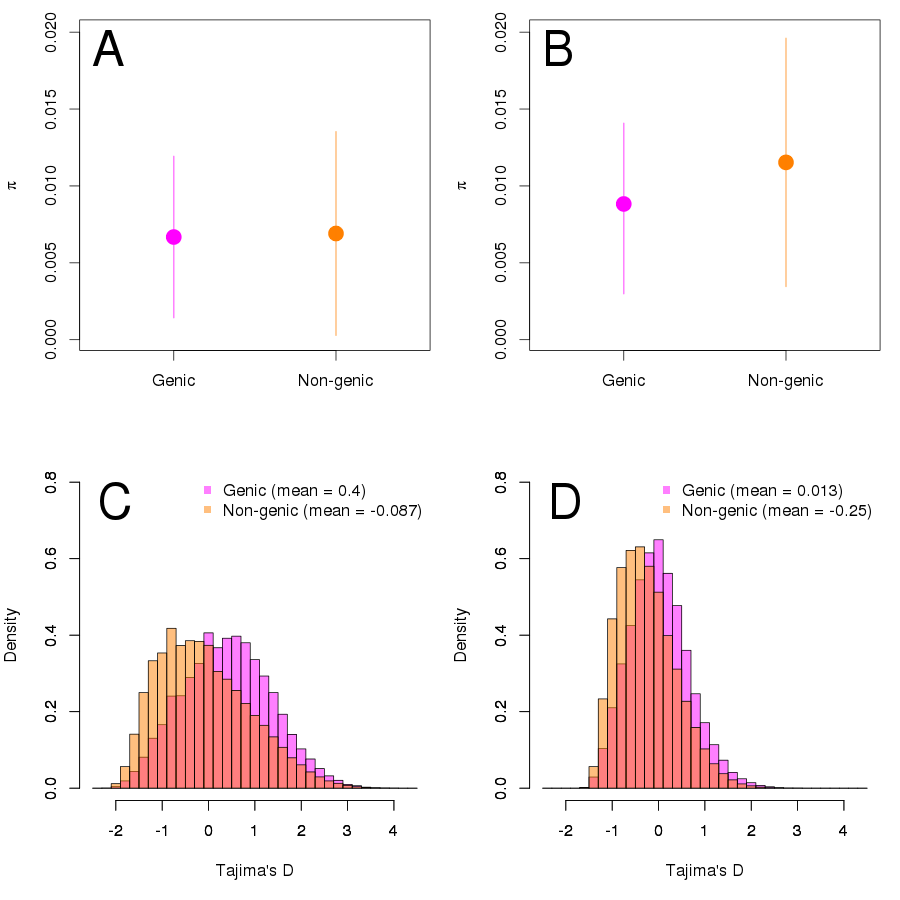
\includegraphics[width=.4\textwidth] {FigsAndFiles/Pi_and_Tajima.png}
\end{center}
\caption{Pairwise diversity $\pi$ (A,B) and Tajimas D (C,D) in 1kb windows from genic and nongenic regions of maize (A,C) and teosinte (B,D). Shown in A and B are means and one standard deviation.   \label{fig:diversity} }
\end{figure}

\subsection{Hard sweeps do not explain diversity differences}
Selection acting to increase the frequency of a new beneficial mutation will leave a signature of reduced diversity at surrounding linked sites \cite{smith1974}.
To evaluate whether patterns of such ``hard sweeps'' could explain observed differences in diversity between genic and non-genic regions of the genome, we compared diversity around missense and synonymous substitutions between \emph{Tripsacum} and either maize or teosinte (Figure
\ref{fig:hardSweeps}).
If a proportion of missense mutations have been fixed due to hard sweeps, diversity around these substitutions should be lower than around synonymous substitutions. 
We observe this pattern around the causative amino acid substitution in the the domestication locus \emph{tga1} (Figure \ref{sFig:tga1}), likely the result of a hard sweep during domestication \cite{wang2005origin, wang2015}.
Genome-wide, however, we observe no differences in diversity between synonymous and missense substitutions in either maize or teosinte.

\begin{figure*}
%\vspace*{.05in}
\centering
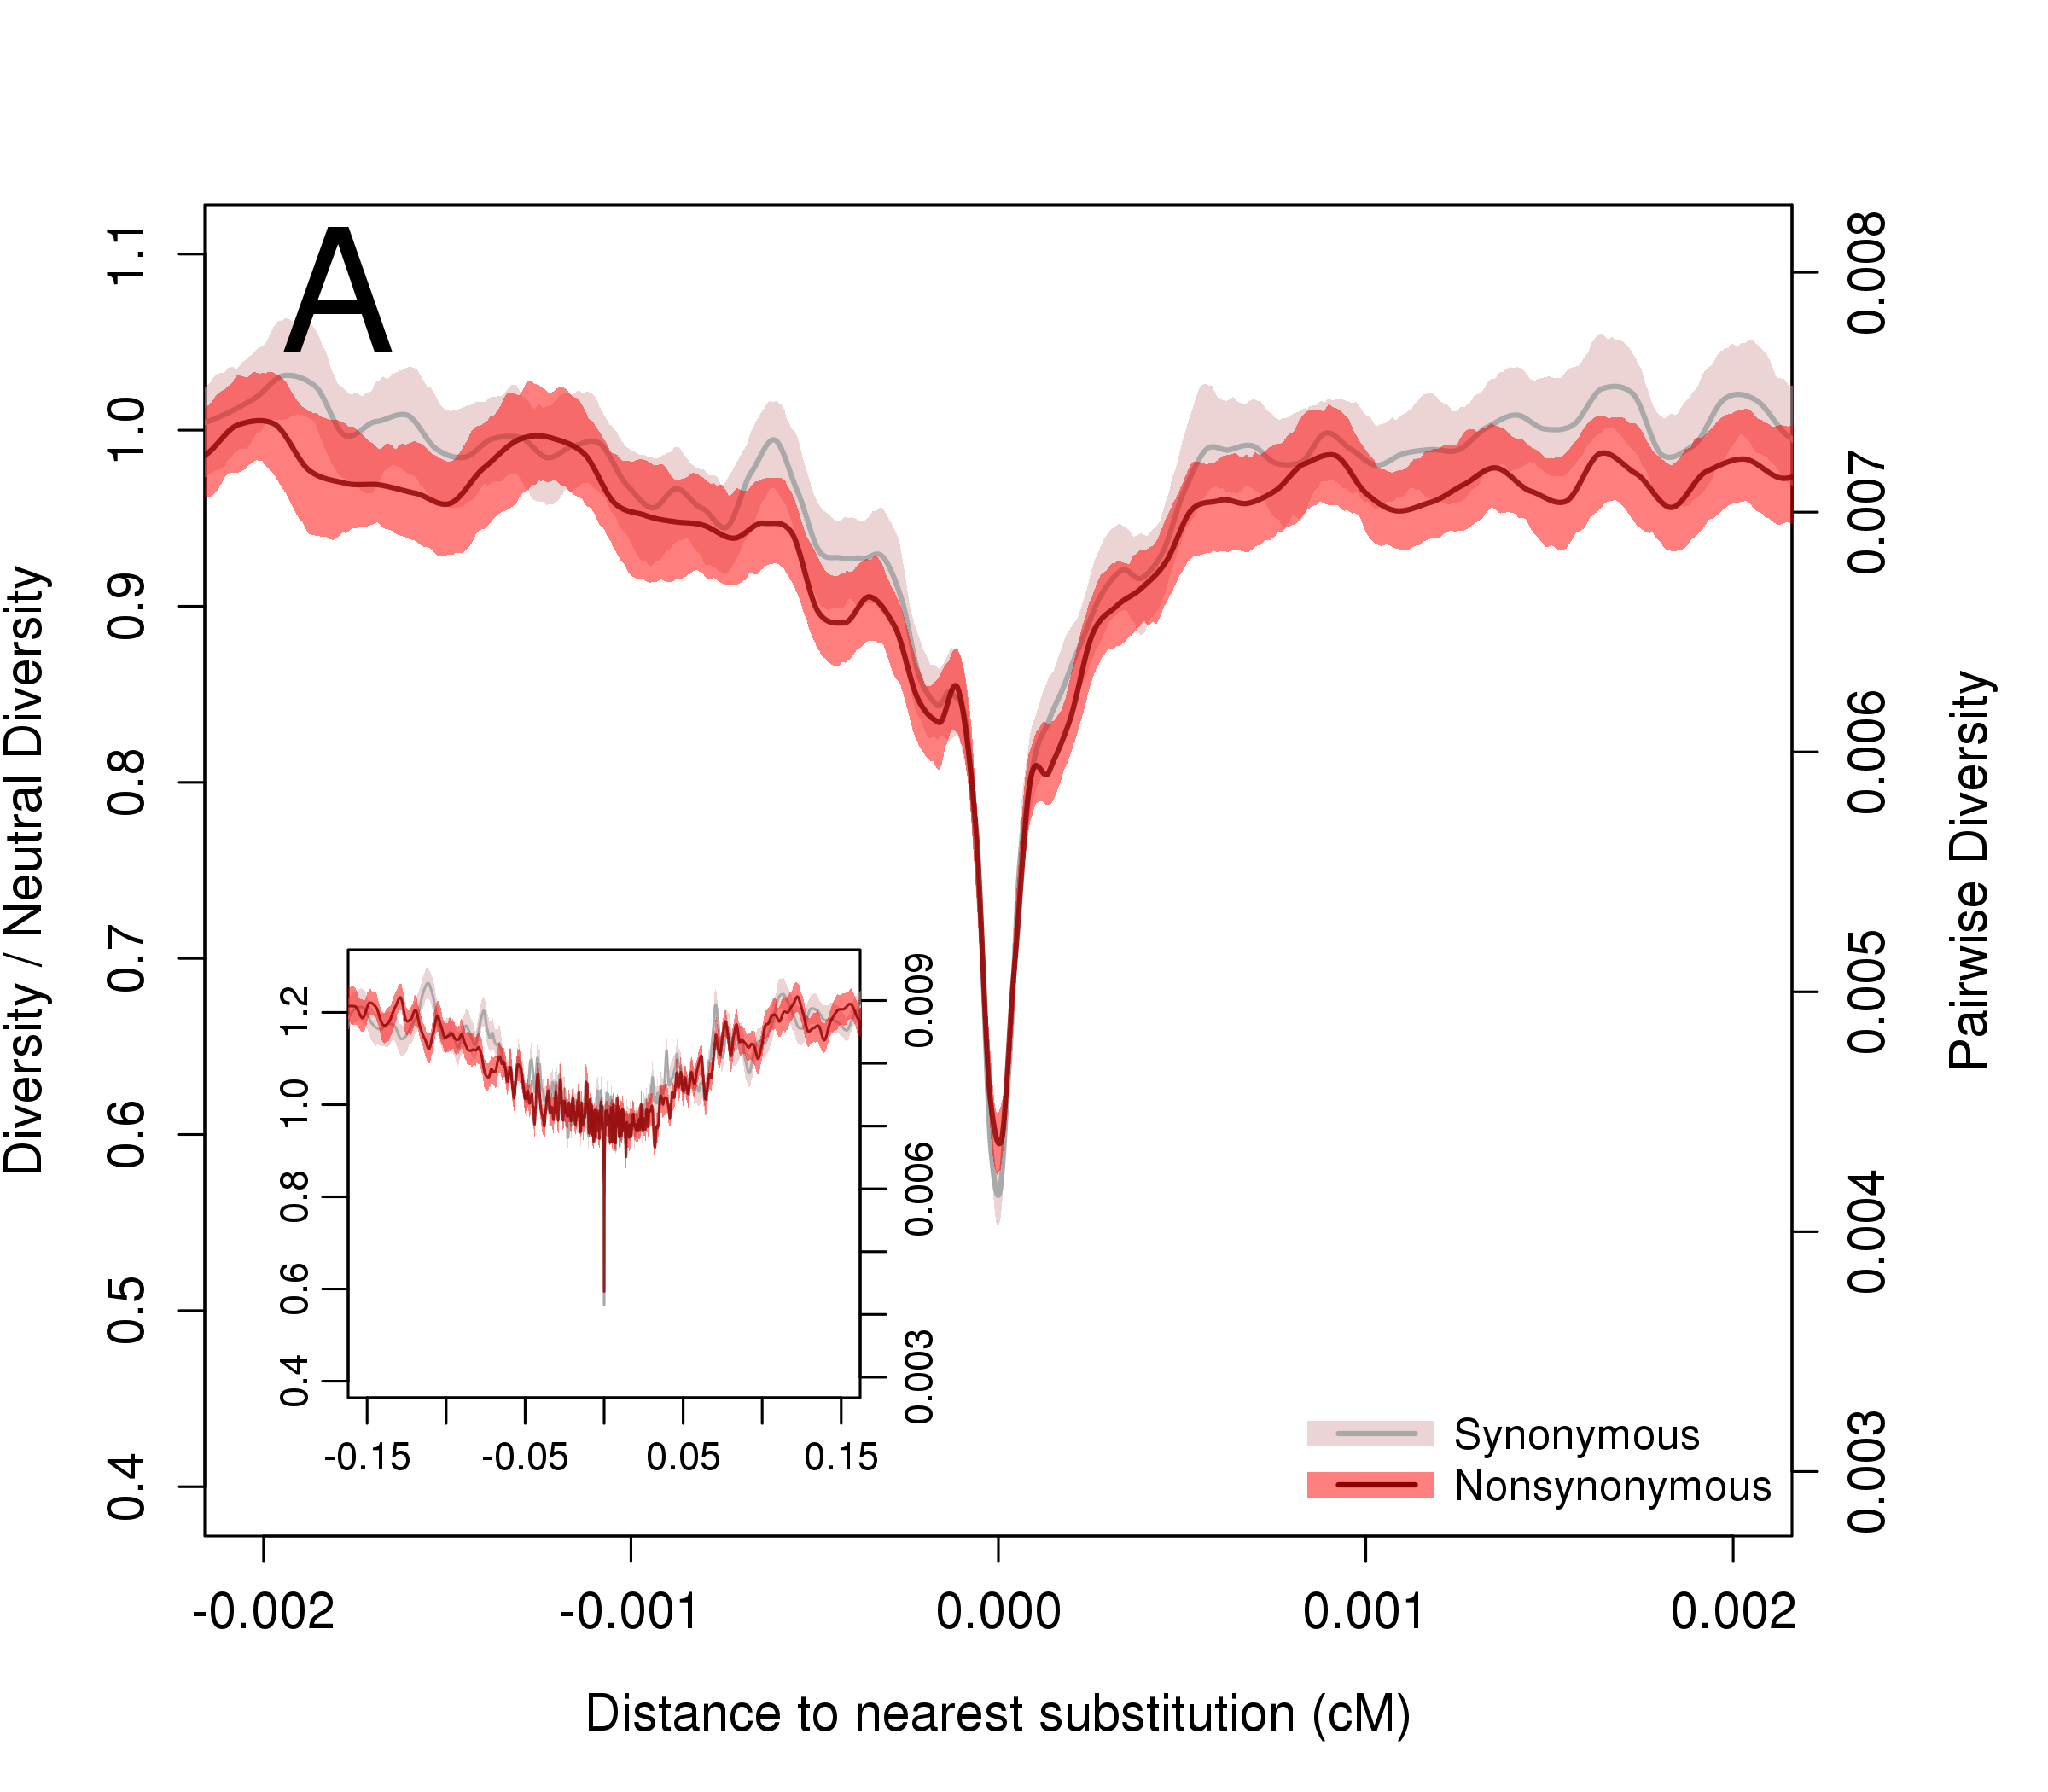
\includegraphics[width=.45\textwidth]{FigsAndFiles/plotDiversity_TvM_Folded2_Significance_Aug}
\hspace{0.05\textwidth} 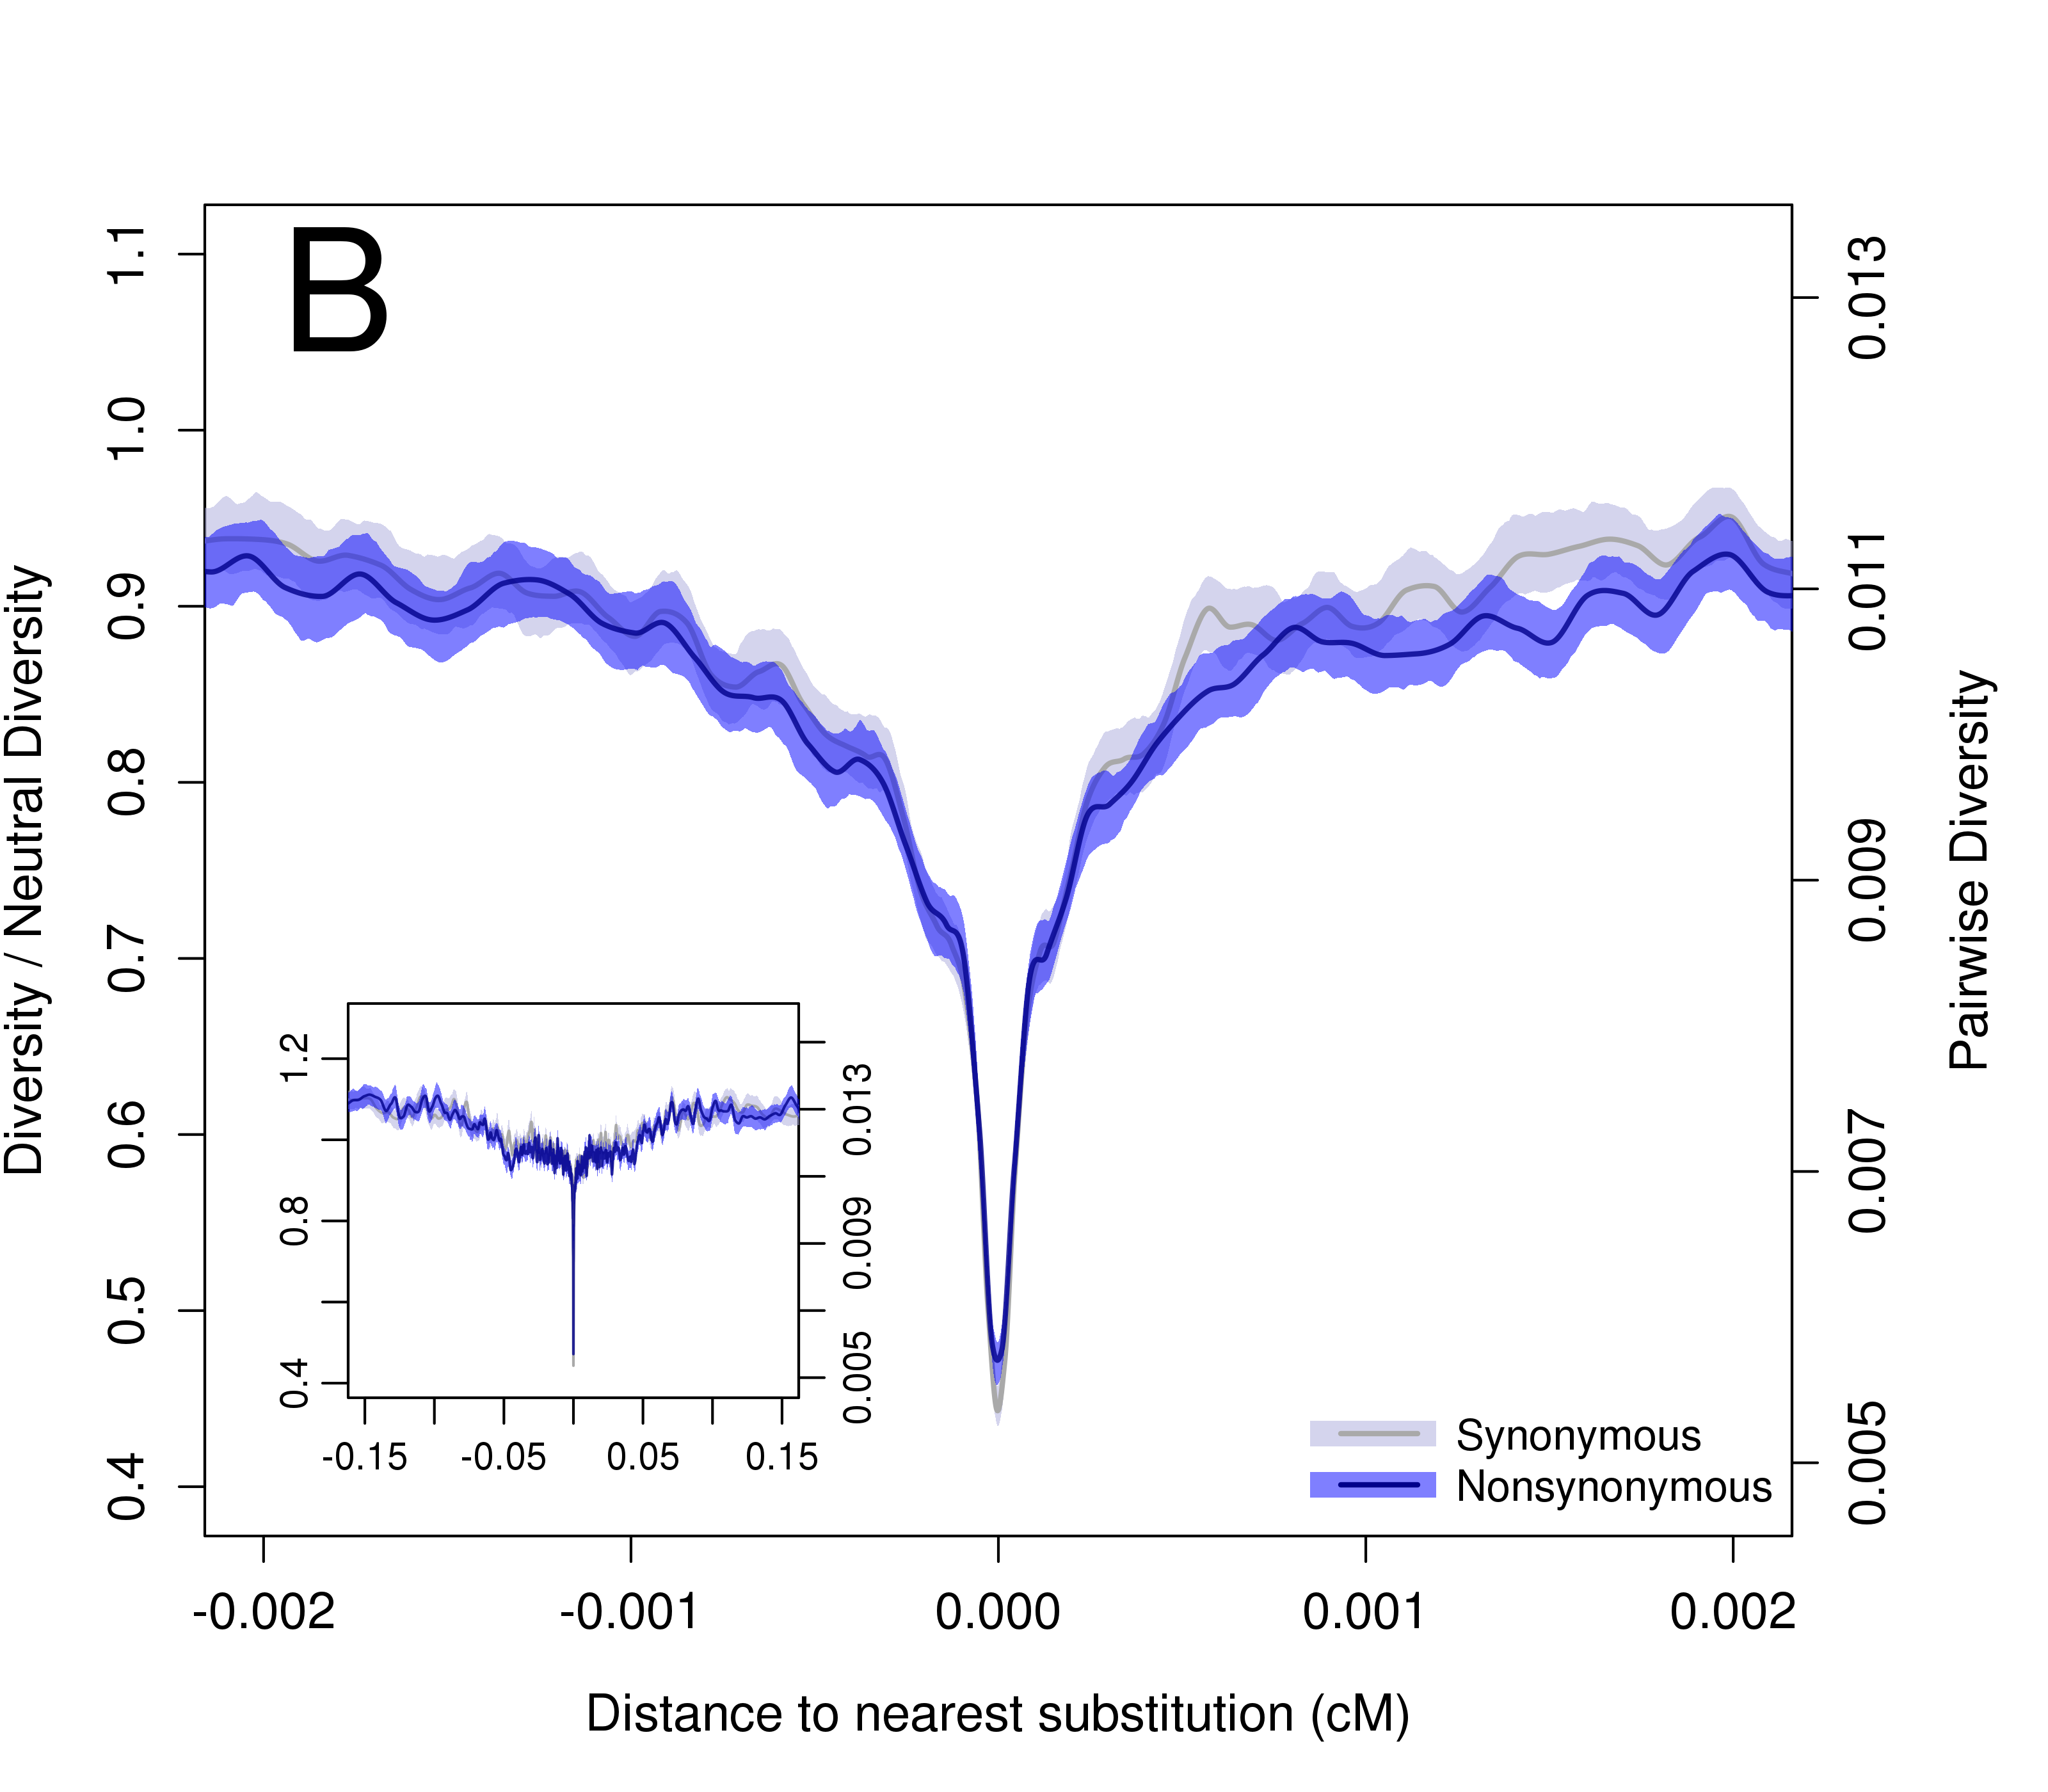
\includegraphics[width=.45\textwidth]{FigsAndFiles/plotDiversity_TvT_Folded2_Significance_Aug}
\caption{Pairwise diversity surrounding synonymous and non-synonymous (missense)
  substitutions in {\bf A} maize and {\bf B} teosinte. Axes show both absolute diversity values (on right) and values relative to mean nucleotide diversity in windows $\geq 0.01 cM$ from a substitution (on left).  Lines depict a loess curve (span of 0.01) and shading represents bootstrap-based 95\% confidence intervals. Inset plots depict a larger range on the x-axis. \label{fig:hardSweeps}}
\end{figure*}

Previous analyses have suggested that this approach may have limited power because a higher proportion of nonsynonymous substitutions will be found in genes under weak purifying selection and thus with higher genetic diversity \cite{enard2014}. 
To address this concern, we took advantage of genomic evolutionary rate profile (GERP) scores \cite{davydov2010}, a measure of evolutionary constraint, calculated across the maize genome \cite{rodgers2015}. 
We re-analyzed substitutions in subsets of genes with the highest and lowest 10\% quantile of mean GERP score, putatively representing genes under the strongest and weakest purifying selection  (Figure \ref{sFig:consUncons}). 
As expected, we see higher diversity around substitutions in genes under weak purifying selection, but we still see no difference between synonymous and missense substitutions in either subset of the data.
Taken together, these data suggest hard sweeps do not play a major role in patterning genic diversity in either maize or teosinte.

\subsection{Diversity is strongly influenced by purifying selection}

Selection can also reduce diversity in functional regions of the genome via removal of deleterious mutations, a process known to as purifying or background selection \cite{charlesworth1993}.
We investigated purifying selection in maize and teosinte by evaluating the reduction of diversity within genes.
Pairwise diversity is strongly reduced within genes for both maize and teosinte (Figure \ref{fig:purify}A) but recovers quickly at sites outside of genes, consistent with the low levels of linkage disequilibrium generally observed in maize \cite{tenaillon2002,chia2012}. 
The reduction in relative diversity is more pronounced in teosinte, however, reaching lower levels in genes and occurring over a wider region.  

Our initial comparison of synonymous and missense substitutions has low power to detect the effects of selection acting on multiple mutations or standing genetic variation, because in such cases diversity is not necessarily reduced \cite{innan2004,messer2013}. 
Such ``soft sweeps'', however, are still expected to occur more frequently in functional regions of the genome and could provide an alternative explanation for the observed reduction of diversity in genes. 
To test this possibility, we performed a genome-wide scan for selection using a method expected to be reasonably sensitive to both hard and soft sweeps \cite{garud2015}. 
After removing genes in the top 20\% of the H12 statistic used to identify targets of selection, we observe that qualitative differences between maize and teosinte in patterns of diversity in and near genes remained unchanged (Figure \ref{sFig:H12}A).

We interpret these combined results as suggesting that purifying selection has left a more pronounced signature in the teosinte genome due to the increased efficacy of selection resulting from differences in effective population size.\jri{weird that this is a 1-sentence paragraph?} 

\begin{figure*}
%\vspace*{.05in}
\centering
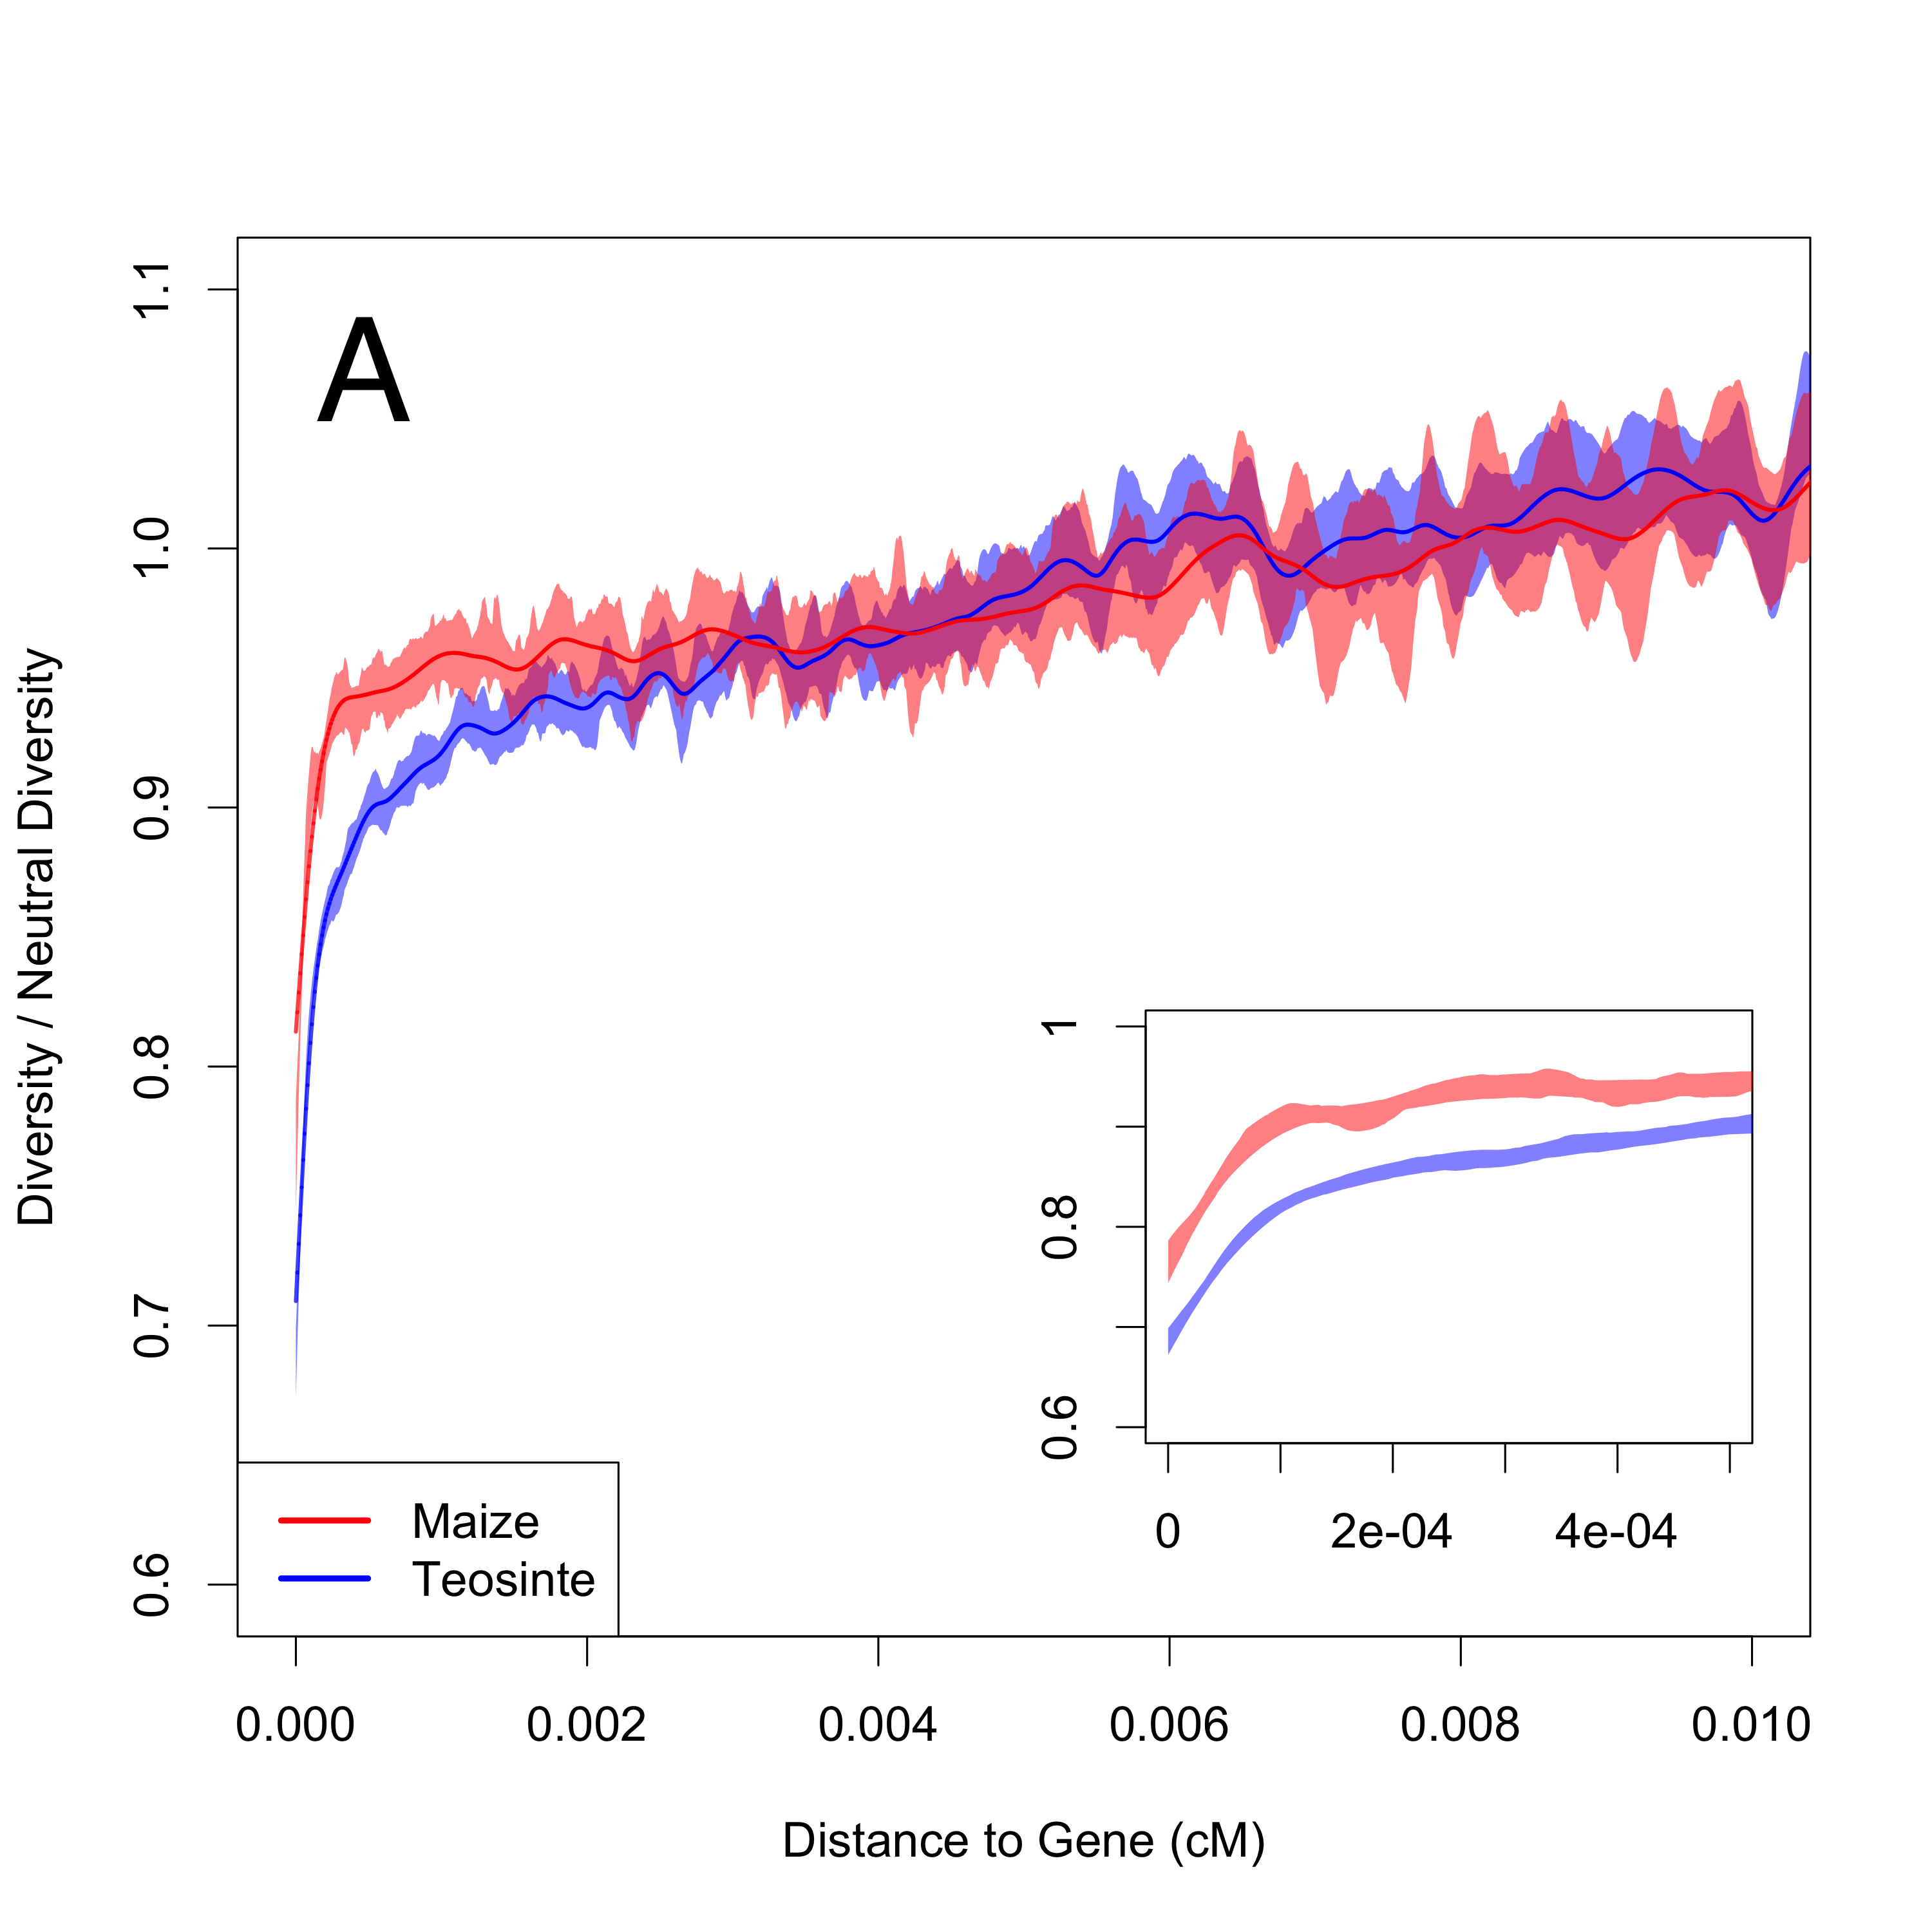
\includegraphics[width=.45\textwidth]{FigsAndFiles/distanceToGene_WithSignificance_Folded2_manuscript.png} 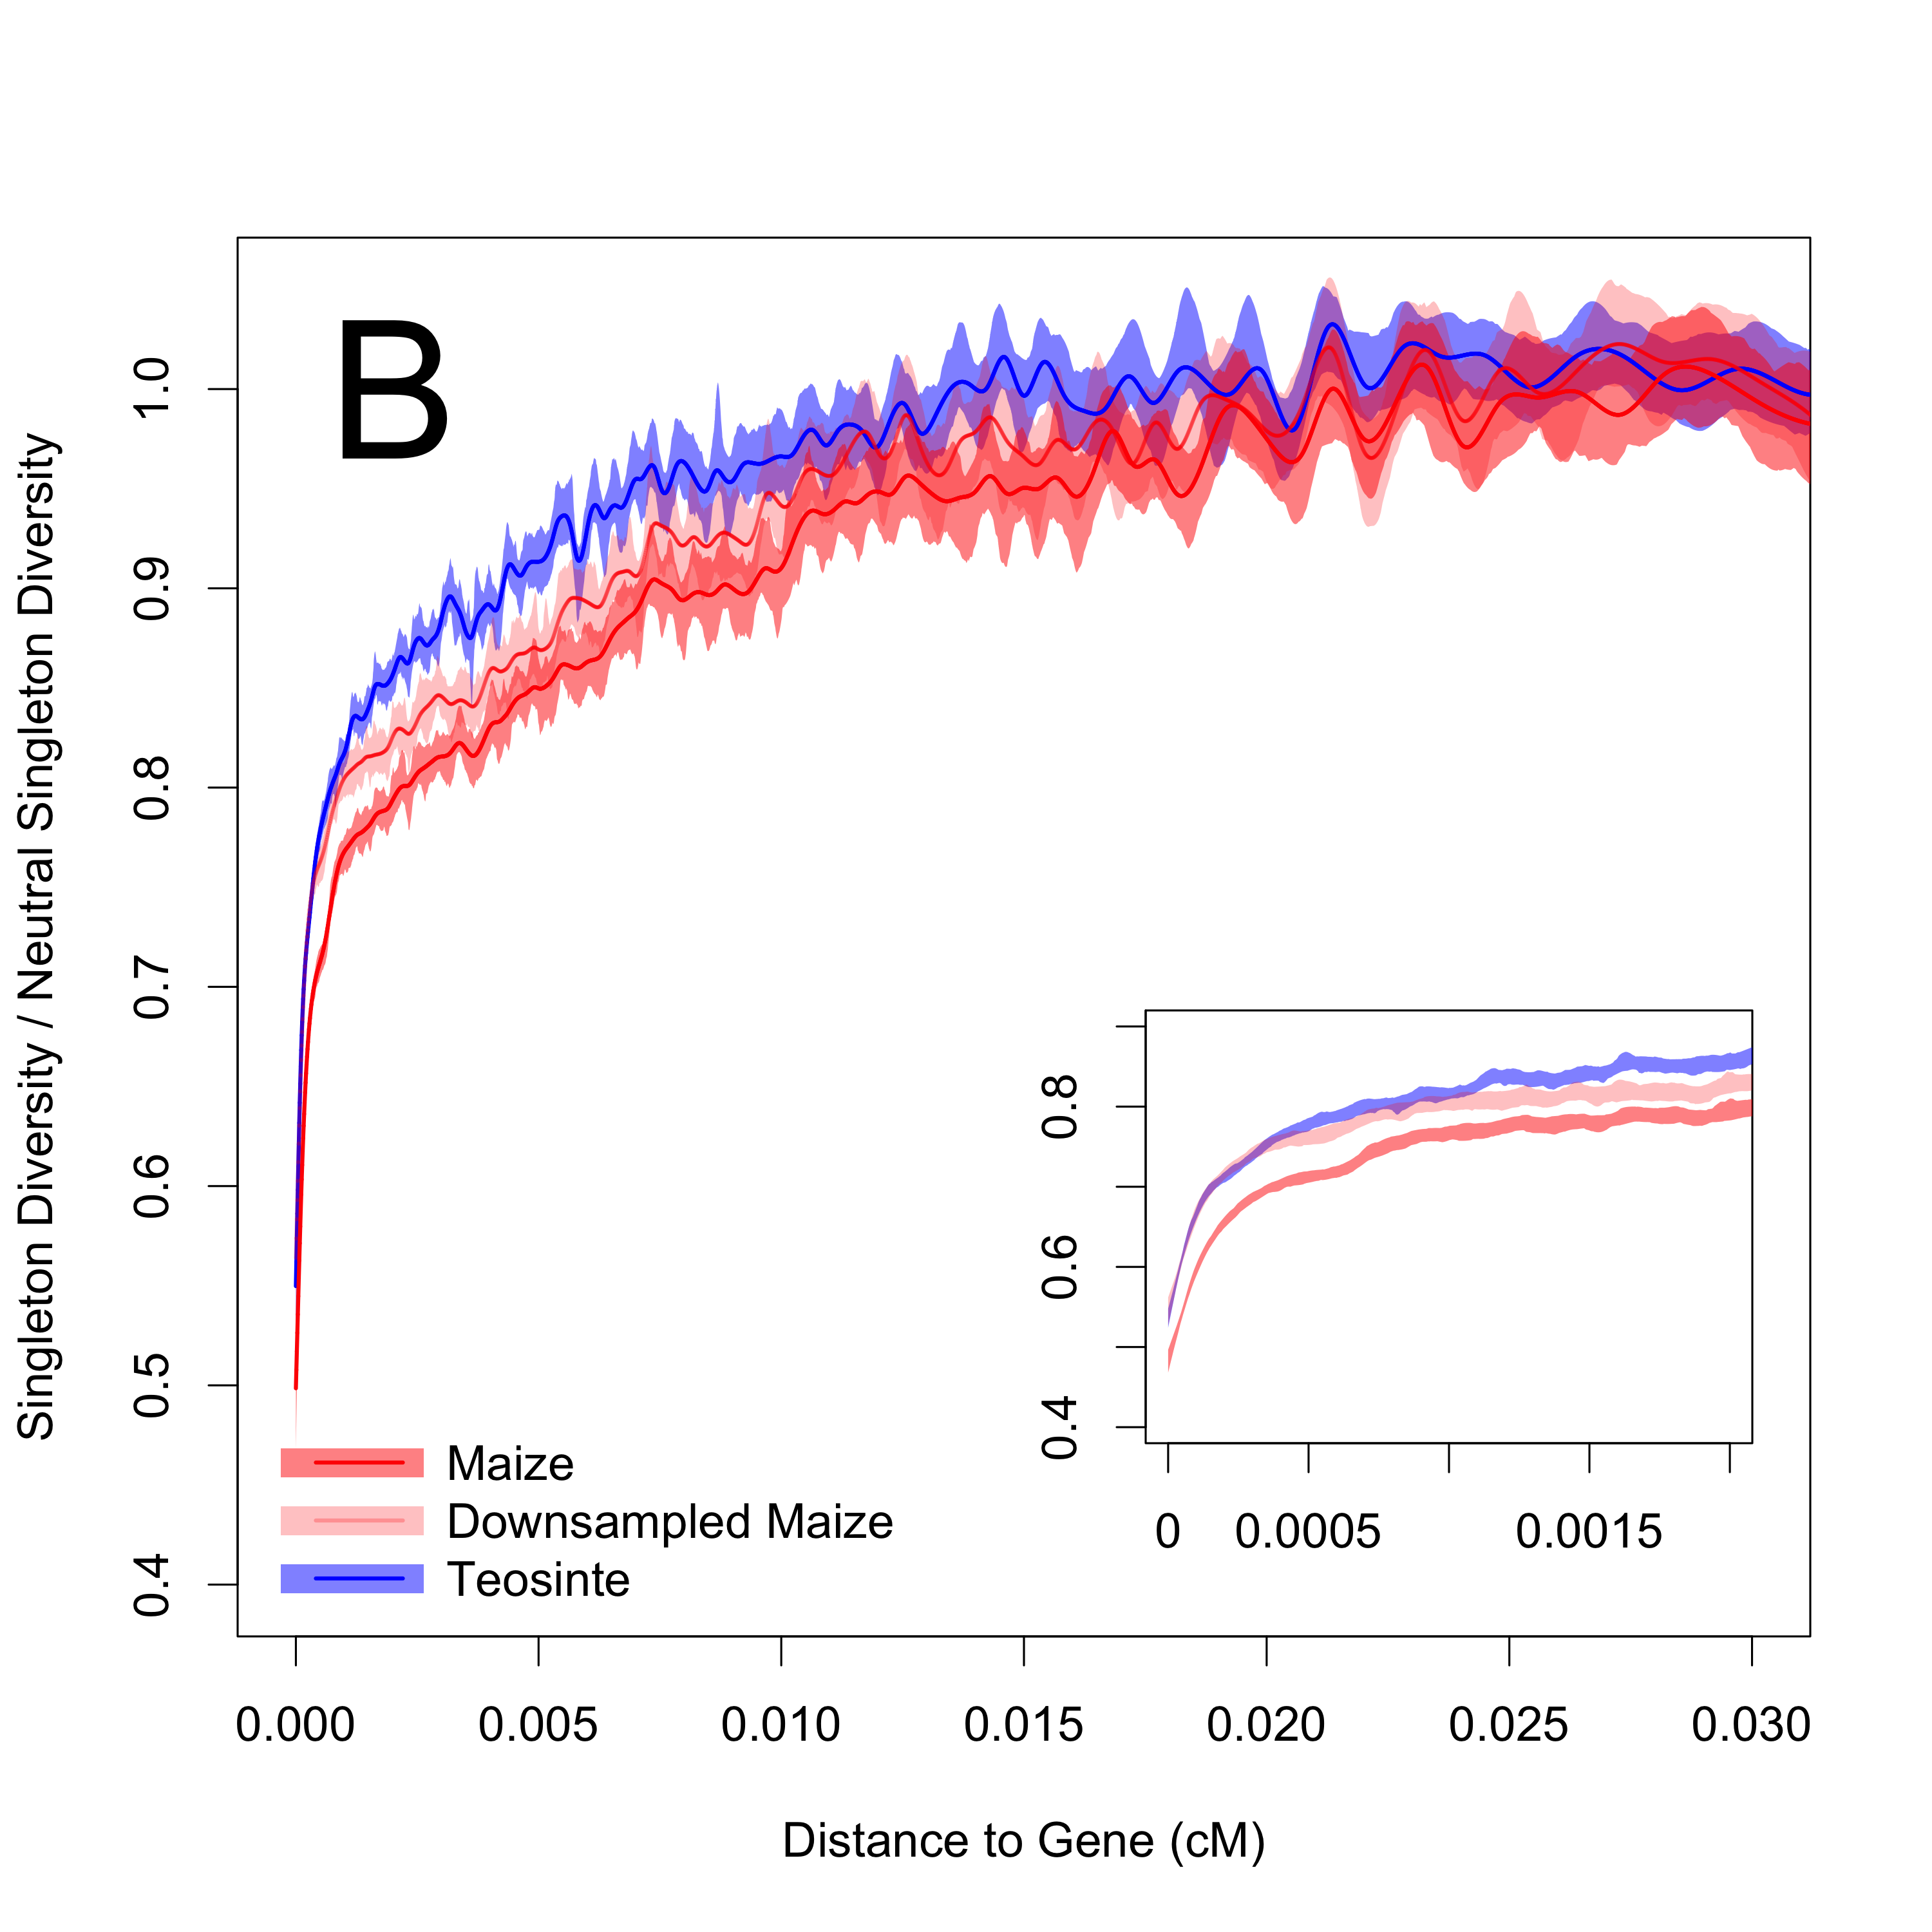
\includegraphics[width=.45\textwidth]{FigsAndFiles/distanceToGene_WithSignificance_Singletons_Downsampled_threeLines_manuscript.png}
\caption{Relative diversity versus distance to nearest gene in maize and teosinte. 
Shown are \textbf{A} pairwise nucleotide diversity and \textbf{B} singleton diversity.  
Relative diversity is calculated compared to the mean diversity in windows $\geq 0.01 cM$ or $\geq 0.02 cM$ from the nearest
gene for pairwise diversity and singletons, respectively. 
  Lines depict cubic smoothing splines with smoothing parameters chosen via generalized cross validation and shading depicts bootstrap-based 95\% confidence intervals.
  Inset plots depict a smaller range on the x-axis. \label{fig:purify}
  }
\end{figure*}

\subsection{Demography of maize domestication}
To explore whether differences in the efficacy of purifying selection between maize and teosinte can be explained by demographic processes, we estimated the parameters of a simple domestication bottleneck model  (Figure \ref{fig:bottleneck}). 
The most likely model estimates an ancestral population mutation rate of $\theta=0.0147$ per bp, which translates to an effective population size of $N_a \approx 123,000$ individuals given the mutation rate \cite{clark2005}.
The maize population splits from teosinte $\approx 15,000$ generations in the past with an initial size of only $\approx 5\% $ of ancestral $N_a$. 
Following domestication we estimate considerable gene flow between the populations: $M_{tm} =  1.1 \times 10^{-5} \times N_a $  migrants per generation from teosinte to maize and $M_{mt} =  1.4 \times 10^{-5} \times N_a$ migrants from maize to teosinte. 
After its split from teosinte our model posits exponential population growth in maize, estimating a final modern effective population size of $N_m \approx 370,000$.

\begin{figure*}
%\vspace*{.05in}
\centering
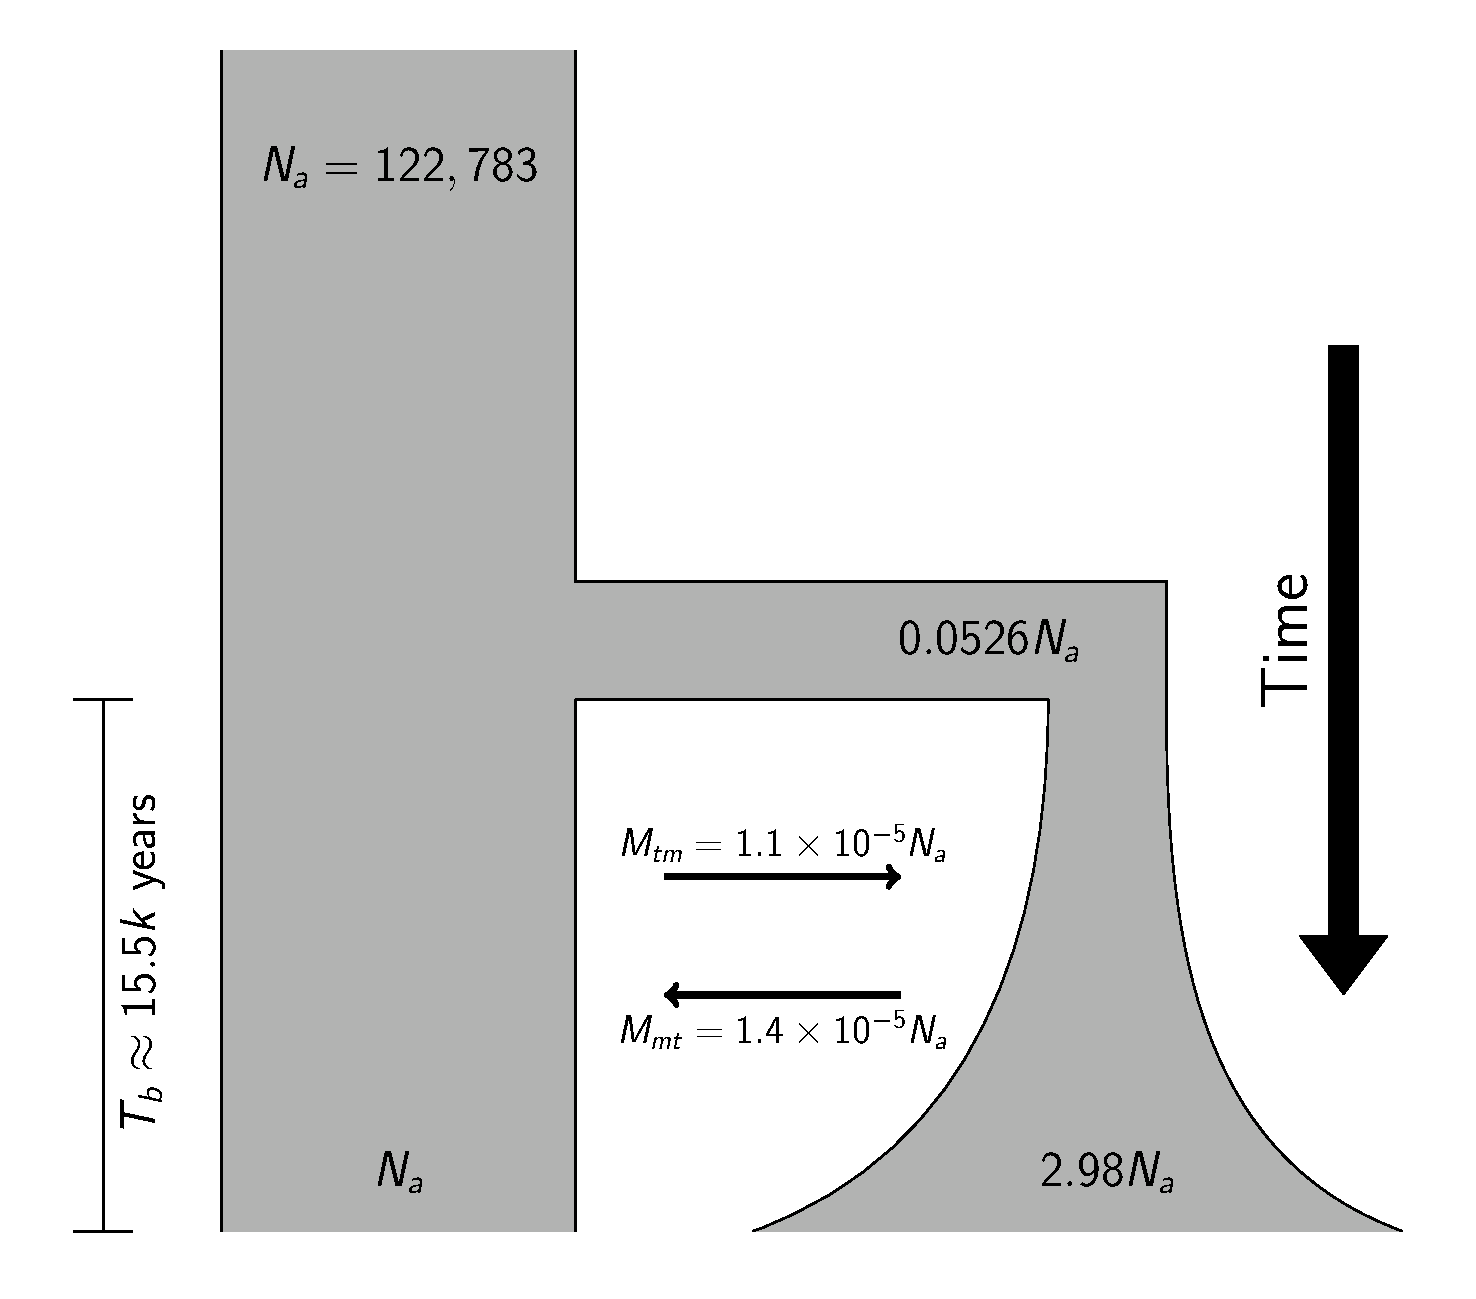
\includegraphics[width=.4\textwidth]{FigsAndFiles/DomesticationModel/domesticationModel.pdf}
\caption{Parameter estimates for a simple bottleneck model of maize domestication. See methods for details. \label{fig:bottleneck} }
\end{figure*}

Because our relatively small sample size limits our ability to characterize the rare variants that are most informative of population expansion, we took advantage of a complementary data set of more than 4,000 maize landraces collected from across the Americas \cite{Hearne2015} to estimate the modern maize effective population size from low frequency variants. 
This analysis yields a much higher estimate of the modern maize effective population size at  $N_m \approx 993,000$.

%MSMC results
%Finally, we reconstructed the demographic history of maize and teosinte using a recently developed coalescent approach \citex that does not require conditioning on a particular model (Figure \X).
%Though this analysis does highlight a potential weakness with our assumption of a constant size for teosinte, it nonetheless is broadly consistent with our simple model,   identifying a clear domestication bottleneck followed by rapid population expansion (Figure \X). 

\subsection{Population expansion leads to stronger purifying selection in modern maize}
Motivated by the rapid post-domestication expansion of maize evident from our demographic analysis, we investigated whether patterns of diversity at low frequency --- and therefore on average younger --- polymorphisms would show similar results in comparisons of maize and teosinte.
We thus repeated our analysis of diversity using alleles present in only a single individual in the sample.
In direct contrast to patterns observed for pairwise nucleotide diversity (Figure \ref{fig:purify}A), diversity of singletons was more strongly reduced in and near genes in maize than in teosinte (Figure \ref{fig:purify}B), even after downsampling our maize data to account for differences in sample size. This relationship was maintained when we analyzed diversity surrounding genes that did not show evidence of hard or soft sweeps according to H12 (Figure \ref{sFig:H12})
Finally, while direct comparison of curves for pairwise and singleton diversity within taxa are consistent with at least some non-equilibrium dynamics in teosinte, these too reveal much stronger differences in maize (Figure \ref{sFig:singletonPi}). %ref. here to MSMC if we use: "as indicated by our coalescent-based demographic analysis"

These results suggest that demographic history and population size change have impacted the efficacy of purifying selection during maize evolution.
In contrast, analysis of singleton diversity around missense and synonymous substitutions (Figure \ref{sFig:singleton}) provides a nearly identical pattern to that shown in Figure \ref{fig:hardSweeps}, providing little support for a substantial increase in the number or strength of hard sweeps occurring in maize.  

\section{Discussion}

%JRI suggestions
%no strong evidence for hard sweeps, even considering constraint (GERP).
%although this is not super powerful test as misses sweeps on noncoding and only has power if substantial proportion of missense sites are swept, much previous evidence argues against hard sweeps in maize.  
%popgen studies of local adaptation \cite{Takuno15062015} and modern breeding \cite{beissinger2014} show importance of standing variation. 
%even in domestication, few fixed differences between maize and teo \cite{hufford2012}, and of domestication loci that have been well studied from a popgen standpoint only one shows hard sweep \cite{wang2015} while there are multiple examples of standing variation \cite{studer2011, wills2013} or selection on multiple mutations \cite{wills2013}. \jri{maybe others? barren stalk 1 (gallavotti 2004)? ramosa 1 (sigmon 2010)? }
%
%this lack of hard sweeps patterning diversity differs from drosophila \citex and capsella \citex and many species with high Ne \jri{cite corbet-detig}. \jri{add something about corbet-dettig results for maize}
%but is consistent with humans \cite{hernandez2011}
%discussion of whether we expect hard vs soft in maize \cite{messer2013population}.
%$\theta_b = 2N\mu_b$ with $mu_b$ being mutation rate of beneficial alleles of selection coefficient s. 
%if $\theta_b > \frac{1}{log{Ns_b}}$ then adaptation from multiple mutations should be common. 
%if  $\theta_b > \frac{1}{log{2Ns_b}}$ then adaptation from standing neutral variation should be common, or if $\theta > \frac{1}{log(1+\frac{2Ns_b}{2Ns_d + 1}}$ for standing deleterious variation with selection coefficient $s_d$. \jri{i think this latter assumes codominance} codominant?) 

%Our findings indicate that hard selective sweeps have not contributed substantially to genome-wide patterns of diversity in maize.
%One known example of positive selection on a non-genic mutation involves the \emph{tb1} locus of maize, which is one of the best characterized examples of positive selection on a ``domestication gene'' in any crop \cite{clark2006}. However, the maize \emph{tb1} allele was already present in teosinte before domestication \cite{studer2011}, so this this example is in agreement with our finding that hard sweeps are rare. The \emph{gt1} locus is another well-characterized case of positive selection operating on standing variation at an enhancer region \cite{wills2013}. Instances of selection on standing variation such as these, often called soft sweeps, may be a major contributor to maize patterns of diversity \cite{beissinger2014}, and this could be part of the explanation as to why hard sweeps appear to be so rare, despite obvious morphological differences between maize and teosinte.

%Unfortunately, our ability to accurately identify soft sweeps, and particularly to distinguish them from hard sweeps, remains limited \cite{innan2004,messer2013}. However, we implemented a scan based on the H12 statistic, which is designed to identify both hard and soft sweeps with reasonable power \cite{garud2015}. Although the goal of this study was not to identify specific sweeps, it may be that the outlier sites distinguished by H12 are primarily composed of soft sweeps instead of hard. Similarly, previous studies scanning for evidence of positive selection in maize \cite{hufford2012} may have picked up primarily evidence of soft sweeps.

%We should additionally note that our observations do not exclude the possibility of infrequent hard sweeps having taken place during maize evolution. In fact, the maize locus \emph{tga1} that has been shown to correspond to a hard sweep at an amino-acid changing mutation \cite{wang2015}. Surrounding \emph{tga1},  our data demonstrate a pattern consistent with a hard sweep. But, our data demonstrate that instances such as this are infrequent. This contrasts sharply with \emph{Drosophila} \cite{sattath2011} and \emph{Capsella} \cite{williamson2014}, where differences in diversity surrounding synonymous and non-synonymous substitutions are clear suggesting hard-sweeps are abundant. However, it agrees with what has been seen for humans \cite{hernandez2011}. 

\subsection{Hard sweeps do not shape genome-wide diversity in maize}

Our findings demonstrate that hard selective sweeps have not contributed substantially to genome-wide patterns of diversity in maize, a result we show robust to concerns about power due to the effects of background selection  \cite{enard2014}. 
Although our approach ignores the potential for hard sweeps in noncoding regions of the genome, a growing body of evidence argues against hard sweeps as the prevalent mode of selection shaping maize variability. 
Population genomic studies of domestication \cite{hufford2012},  local adaptation \cite{Takuno15062015} and modern breeding \cite{beissinger2014} all support the importance of standing variation as the primary source of adaptive variation. 
Even among well-characterized domestication loci, only a single locus shows evidence of a hard sweep on a missense mutation \cite{wang2015}, but several are consistent with selection on standing variation \cite{studer2011,gallavotti2004role} or multiple mutations \cite{wills2013}.

The lack of hard sweeps patterning diversity differs from drosophila \cite{sattath2011} and capsella \cite{williamson2014},but is consistent with humans \cite{hernandez2011}. In a related study, \cite{corbett2015} showed that selection tends to have an elevated impact on reducing diversity in species with large population size compared to small. This may explain why maize and humans, both bottlenecked species, show similar patterns while drosophila and capsella behave differently. \textcolor{red}{However, we also do not observe abundant hard sweeps in teosinte, which calls this hypothesis into question.}

Another possibility is that maize and teosinte don't show evidence of abundant hard sweeps because instead positive selection tends to operate in the form of soft sweeps. The theory of when soft sweeps are expected was worked out by \cite{messer2013population}. They showed that for $\theta_b = 2N\mu_b$, where $\mu_b$ is the mutation rate of beneficial alleles with selection coefficient $s_b > 0$, if $\theta_b > \frac{1}{log({Ns_b})}$, then soft sweeps in the form of adaptation from multiple mutations should be common. Conversely, for neutral sites that somehow become beneficial (e.g. change in environment), if $\theta_b > \frac{1}{log({2Ns_b})}$ then soft sweeps in the form of adaptation from standing neutral variation should be common. Alternatively, for previously deleterious sites that become beneficial, if $\theta > \frac{1}{log \left(1+\frac{2Ns_b}{2Ns_d + 1} \right)}$, where $s_d$ is the previous selection coefficient, soft sweeps again the form of adaptation from standing variation should be common. The implications of this theory are that soft sweeps are common when $\theta_b \geq 1$ \cite{messer2013population}, which can be achieved through a large population size or a high mutation rate. The best estimate of mutation rate for maize is $\mu = 3 \times 10^{-8}$  \cite{clark2005}, which implies that soft sweeps should be common if population size is $\geq$ 16.67 million. \textcolor{red}{According to our demographic analysis, this is larger than that of teosinte but, as discussed below, not out of the question for modern maize.}
\subsection{Demography of domestication}

Although many other authors have investigated the demography of maize domestication \cite{eyre1998, tenaillon2004selection, wright2005}, these  efforts relied  exclusively genic polymorphisms and have made a number of limiting assumptions about the demographic model.  
We show that diversity within genes has been strongly reduced by the effects of linked selection, making genic data inappropriate for estimating demography.
Because levels of diversity alone do not allow independent inference of the strength and duration of a bottleneck \cite{tenaillon2004selection}, previous investigations have instead estimated the ratio of these parameters.  
We have overcome this limitations through the use of the full joint SFS of maize and teosinte and consideration of a more realistic model of exponential growth, enabling us to estimate for the first time the strength of the domestication bottleneck.  
Given that modern maize exhibits $\approx 80\%$ of the diversity of teosinte, our estimate that  the effective population size of the initial maize  population was only $\approx 5\%$ of the ancestral teosinte population seems surprisingly low.
The impact of a strong domestication bottleneck is likely ameliorated to some degree by  maize-teosinte gene flow and the rapid post-domestication growth estimated in our model.   

Another surprising result from our model is the estimation of the timing of domestication.
Although we estimate the maize population split $\approx 5,000$ years earlier than previous molecular \cite{matsuoka2002} or archaelogical \cite{piperno2009starch} estimates, we do not interpret these results as strongly conflicting.
We first note that the timing of the genetic split between populations likely preceded the anatomical changes that can be identified in the archaeological record. 
We also caution, however, that our estimate may be inflated by population structure as our geographically diverse sample may include populations diverged from those that gave rise to maize.

Although we estimate that the modern effective size of maize is three times that of teosinte, the small size of our sample dramatically reduces our power to identify low frequency alleles most sensitive to rapid population growth \cite{keinan2012}.  
A better estimate of the effective size of modern maize comes from our analysis of singleton diversity in a large sample of maize landraces \cite{Hearne2015}.
These data suggest a modern effective size of nearly 1 million, nearly eight times higher than modern teosinte.
Nonetheless, missing data, sample size, and ascertainment bias in the genotyping data all bias this estimate downward as well.
We can, however, get reasonable estimates of the census size of modern maize.
There are 47.9 million ha of open-pollinated maize in production \cite{cimmyt1999}, with a lower limit of 25,000 individuals planter per hectare \cite{baden2001culture}.
Using this lower bound on planting density, ignoring all industrial maize agriculture, and even assuming the effective size is only 0.1\% of the census size, this still implies a modern effective population size of more than one billion.
Clearly, the effective size of modern maize is extremely large.

\subsection{Demography influences the efficiency of purifying selection}
The observation that pairwise diversity in maize is less affected by the distance to the nearest gene than in teosinte is reasonable from a long-term evolutionary standpoint. Purifying selection works more efficiently in a large population than in a small one \cite{kimura1984}, so this observation likely reflects that prediction. Since maize bottlenecked before recovering exponentially, the average $N_e$ of maize over the previous several thousand generations is much smaller than that of teosinte. Therefore, our observation shows that purifying selection in maize has not purged deleterious alleles, or the neutral alleles they are linked to, as effectively as in teosinte.

The reversal of this trend when we analyze only singleton diversity instead of pairwise diversity stands out as a notable. Every mutation begins as a singleton (an allele present in only one individual), and therefore singletons are, on average, the youngest class of alleles that can be observed. Unlike pairwise patterns of diversity, which are most heavily influenced by intermediate frequency alleles based on the definition of $\pi$ \cite{nei1979}, singleton diversity is most influenced by recent patterns of evolution. Hence, because our demographic estimation indicates dramatic expansion of maize $N_e$ in the recent past, we expect for purifying selection to presently operate more efficiently in maize than in teosinte. This observation is very clearly demonstrated by the fact that singleton diversity in maize is more impacted by the distance to the nearest gene than it is in teosinte, as was shown in Figure \ref{fig:purify}.

A consequence of the inefficient purifying selection that maize experienced during its bottleneck is likely that it harbors more weakly deleterious alleles segregating at intermediate frequency than does teosinte. This could be a part of the explanation of why maize inbreds have continued to improve over the past several decades \cite{meghji1984}; if deleterious alleles tend to be recessive and are particularly frequent, they will have ample opportunities to display their phenotypes in inbreds. Our results also demonstrate that recent purifying selection in maize has become much more effective, potentially explaining the ongoing improvement of these inbreds as maize lines are continuously selected. Additionally, the large $N_e$ of modern maize compared to modern teosinte implies that for new mutations, selection will operate much more efficiently in maize.

 Importantly, our estimation of the parameters of the maize domestication bottleneck contribute to the understanding of how the demography of crop domestication can impact crop diversity. The bottleneck-effects from a sudden collapse in population size have been well studied and are known to impact crops for thousands of generations. Complementing this knowledge, our results demonstrate that the rapid expansion experienced by many crops after domestication can also have a profound influence on patterns of diversity, and the effects of this expansion should be accounted for as important contributors to long-term evolution. \jri{this is sorta fluff and doesn't say much} 

\jri{need paragraph also talking about how this is important for considering impact of linked selection. cite some recent human papers that are considering both demography and linked selection, but also a number of plant papers that e.g. estimate the DFE from current data or just use the sny/nonsyn graphs and ignore recent demographic history. is capsella a good example? } \textcolor{red}{I agree about this paragraph, but I ran out of time to address. Leave like this and I'll add more after Sept. 11.}

\begin{materials}

  \subsection{BASH, R, and Python scripts}
All scripts used for analysis are available in an online repository at \textcolor{red}{REPO ADDRESS HERE.} 

\subsection{Plant materials}
We made use of published sequences from inbred accessions of teosinte (Z. \emph{mays} ssp. \emph{parviglumis}) and maize landraces from the Maize HapMap3 panel as part of the Panzea project (bam files are available at \textcolor{red}{/iplant/home/shared/panzea/hapmap3/bam\_internal/v3\_bams\_bwamem}) \cite{chia2012, lemmon2014,hapmap3}. 
From these data, we removed 4 teosinte individuals that were not ssp. \emph{parviglumis} or appeared as outliers in an initial principal component analysis conducted with the package adegenet \cite{jombart2011} (Figure \ref{sFig:PCA}), leaving 13 teosinte and 23 maize that were used for all subsequent analyses (Table \ref{sTab:list}). We also utilized a single tripsacum (\emph{T. dactyloides}) individual as an outgroup (bam file available at \textcolor{red}{/iplant/home/shared/panzea/hapmap3/bam\_internal/v3\_bams\_bwamem}).

\subsection{Physical and genetic maps}
Sequences were mapped to the maize B73 version 3 reference genome \cite{schnable2009} (ftp://ftp.ensemblgenomes.org/pub/plants/release-22/fasta/zea\_mays/dna/) as described by \cite{hapmap3}. All analyses made use of uniquely mapping reads with mapping quality score $\geq  30$ and bases with base quality score $\geq 20$; quality scores around indels were adjusted following Li \emph{et al.} \cite{li2011statistical}.
We converted physical coordinates to genetic coordinates via linear interpolation of the previously published 1cM resolution NAM genetic map \cite{glaubitz2014}. 

\subsection{Estimating the site frequency spectrum}
We estimated both the genome-wide site frequency spectrum (SFS) as well as a separate SFS for genic (within annotated transcript) and intergenic ($\geq 5kb$ from a transcript) regions. 
We used the biomaRt package \cite{durinck2009,durinck2005} of R \cite{R2014} to parse annotations from genebuild version 5b of AGPv3. 
We estimated single population and joint SFS with the software ANGSD \cite{korneliussen2014}, including all positions with at least one aligned read in $\geq 80\%$ of samples in one or both populations.
We assumed individuals were fully inbred and treated each line as a single haplotype. Because ANGSD cannot calculate a folded joint SFS, we first polarized SNPs using the maize reference genome and then folded spectra using $\delta\alpha\delta{i}$ \cite{gutenkunst2009}.

\subsection{Demographic inference}
We used the software $\delta\alpha\delta{i}$ \cite{gutenkunst2009} to estimate parameters of a domestication bottleneck from the joint maize-teosinte SFS, using only sites $>5 kb$ from a gene to ameliorate the effects of linked selection.
We modeled a teosinte population of constant effective size $N_a$, that at time $T_b$ generations in the past gave rise to a maize population of size $N_b$ which grew exponentially to size $N_m$ in the present (Figure \ref{fig:bottleneck}).
The model includes migration of $M_{mt}$ individuals each generation from maize to teosinte and $M_{tm}$ individuals from teosinte to maize.  We estimated $N_a$ using $\delta\alpha\delta{i}$'s estimation of $\theta=4N_a\mu$ from the data and a mutation rate of $\mu = 3 \times 10^{-8}$ \cite{clark2005}. 
We estimated all other parameters using 1,000 $\delta\alpha\delta{i}$ optimizations and allowing initial values between runs to be randomly perturbed by a factor of 2.  
Optimized parameters along with their initial values and upper and lower bounds can be found in table \ref{sTab:dadi}. We report parameter estimates from the optimization run with the highest log-likelihood.

We further made use of a large genotyping data set of more than 4,000 maize landraces \cite{Hearne2015} to estimate the modern maize $N_e$ from singleton counts.
We filtered these data to include only SNPs with data in $\geq 1,500$ individuals, and then projected the SFS down to a sample of 500 individuals by sampling each marker without replacement 1,000 times according to the observed allele frequencies.
We then estimated $N_e$ from the data assuming $\mu = 3 \times 10^{-8}$ \cite{clark2005} and the relation  $4N_e\mu = \frac{S}{L}$ \cite{fu1993}, where where $S$ is the total number of singleton SNPs and $L$ is the total number of SNPs in the dataset.

%%%Shorten if we include MSMC
%Finally, MSMC \cite{schiffels2014} was employed to complement our model-based demographic inference. 
%Using six each of maize and teosinte
%The analyses were run for the following two groups: six maize haplotypes (BKN022, BKN025, BKN029, BKN030, BKN031, BKN033) and six teosinte haplotypes (TIL01, TIL03, TIL09, TIL10, TIL11 and TIL14).
%SNPs were called in ANGSD \cite{korneliussen2014} with the SNP p value set as $1e-6$.
%As the samples are highly inbred, each individual was treated as one haplotype.
%Only Sites with mapping quality bigger than $30$, base quality over $20$ and depth between half and twice of its mean depth were chosen for the analyses, and the residual heterozygous sites were removed from the analyses.
%In addition, as the maize genome contains a large body of repetitive regions \cite{schnable2009}, we used Heng Li's software SNPable (\href{<url>}{<http://lh3lh3.users.sourceforge.net/snpable.shtml>}) to mask out genomic regions, on which short sequencing reads are not uniquely mapped.
%The mappability mask file was generated by cutting the maize genome with $1bp$ shift each time into the $100bp$ single-end reads, which were then mapped back to the maize B73 reference genome \cite{schnable2009}.
%The sites with the majority of overlapping $100$-mers mapped uniquely without one mismatch were called the "SNPable" sites and used for the MSMC analyses.
%The pattern parameter $20\times2+20\times4+10\times2$ was used for the population size inference.

\subsection{Diversity}
We made use of the software ANGSD \cite{korneliussen2014} for diversity calculations and genotype calling. 
We calculated diversity statistics in maize and teosinte in 1 kb non-overlapping windows using filters as described above for the SFS. 
We used allele counts to estimate the number of singleton polymorphisms in each window, and used binomial sampling to create a second maize data set down-sampled to have the same number of samples as teosinte.
We called genotypes in maize, teosinte, and \emph{Tripsacum} at sites with a SNP p-value $<10^{-6}$ and when the genotype posterior probability $>0.95$.
We identified substitutions in maize and teosinte as all sites with a fixed difference with \emph{Tripsacum} and $\leq 20\%$ missing data. 
Substitutions were classified as synonymous, missense, or noncoding using the ensembl variant effects predictor \cite{mclaren2010}.
For each window with $\geq 100bp$ of data we computed the genetic distance between the window center and the nearest synonymous and missense substitution as well as the genetic distance to the center of the nearest gene transcript.  

\subsection{Selection scan}
We scanned the genome to identify sites that have experienced recent positive selection using the H12 statistic \cite{garud2015} in sliding windows of 200 SNPs with a step of 25 SNPs.


\end{materials}

\begin{acknowledgments}
We are indebted to Graham Coop and Simon Aeshbacher for their constructive input during this study. We thank Robert Bukowski and Qi Sun for providing early-access data from maize HapMap3. Funding was provided by NSF Plant Genome Research Project 1238014.
\end{acknowledgments}

\bibliography{Reference}
\bibliographystyle{pnas}
\onecolumn
\section*{Supporting Information}
\renewcommand\thefigure{S\arabic{figure}}    
\setcounter{figure}{0}


\begin{figure}
  \begin{center}
    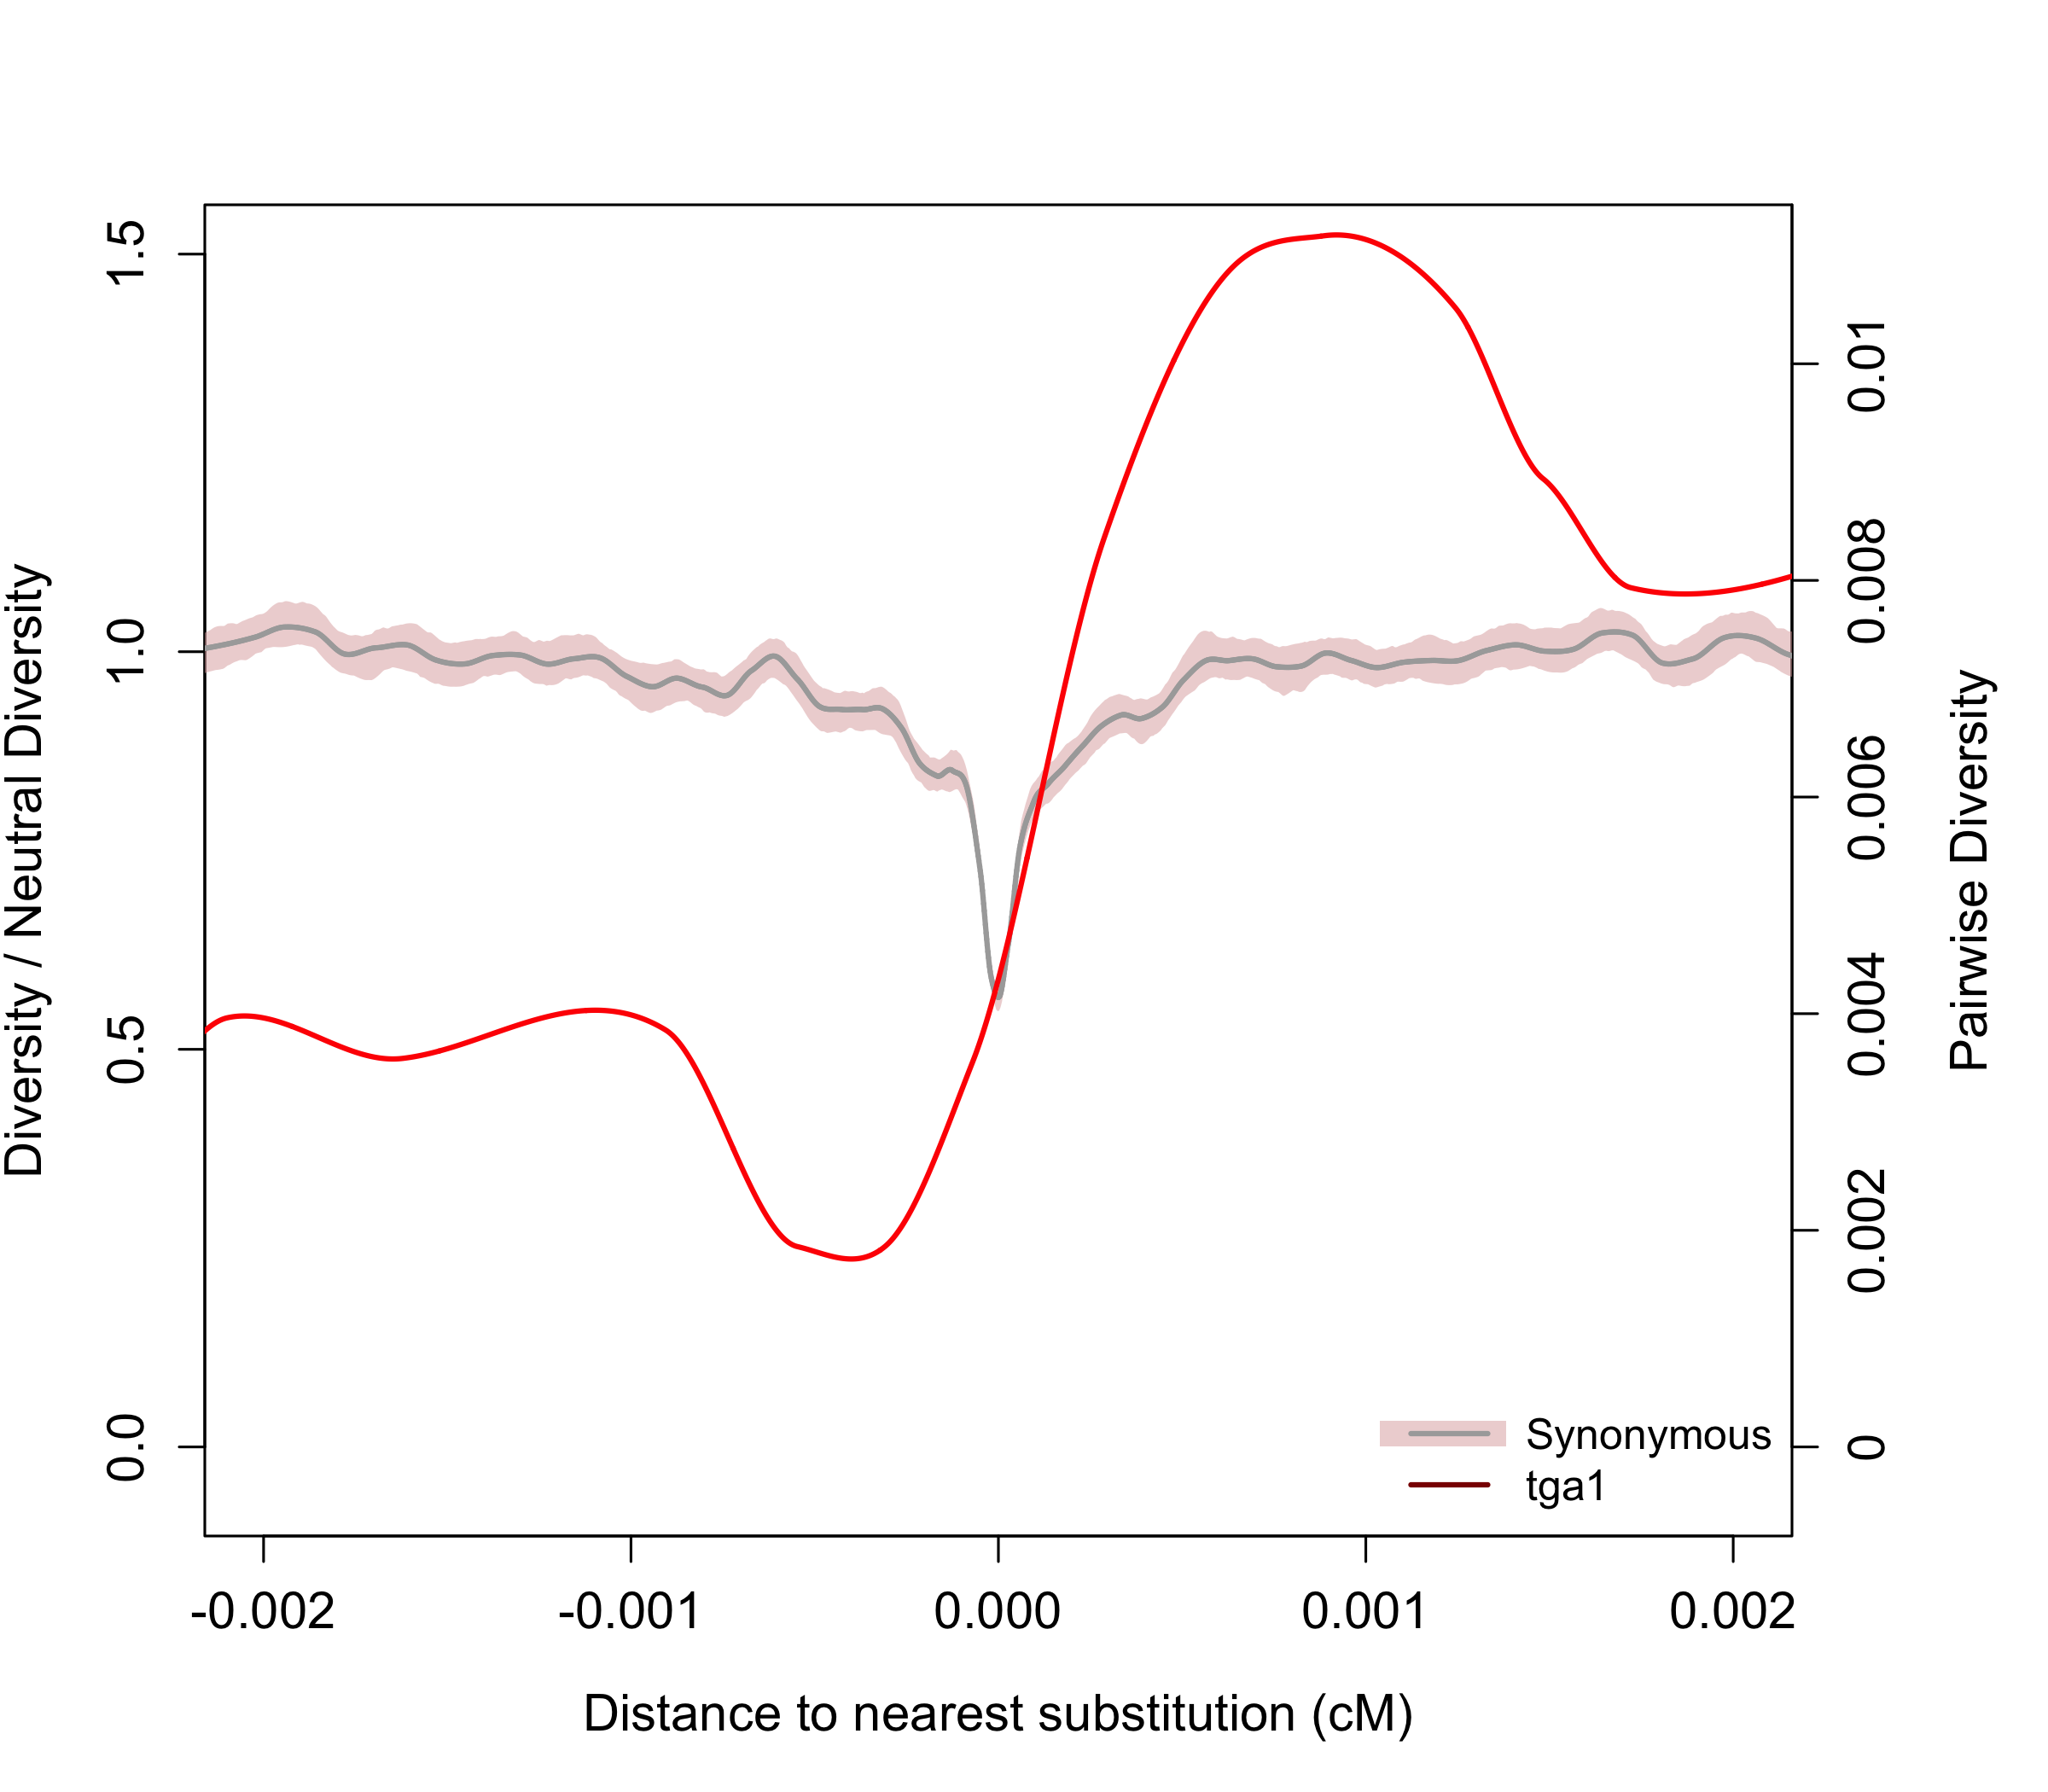
\includegraphics[width=.85\textwidth]{FigsAndFiles/plotDiversity_TvM_Folded2_Significance_tga1Supp_June.png} \\
    \end{center}
\caption{Diversity surrounding the causitive polymorphism at the \emph{tga1} locus is plotted. Since this is only one gene, the large amount of noise compared to our average plots is expected. However, notice that diversity precisely at the causitive polymorphism is reduced and a recovery of diversity is observed away from that site. \label{sFig:tga1}}
\end{figure}
\clearpage


\begin{figure}
  \begin{center}
    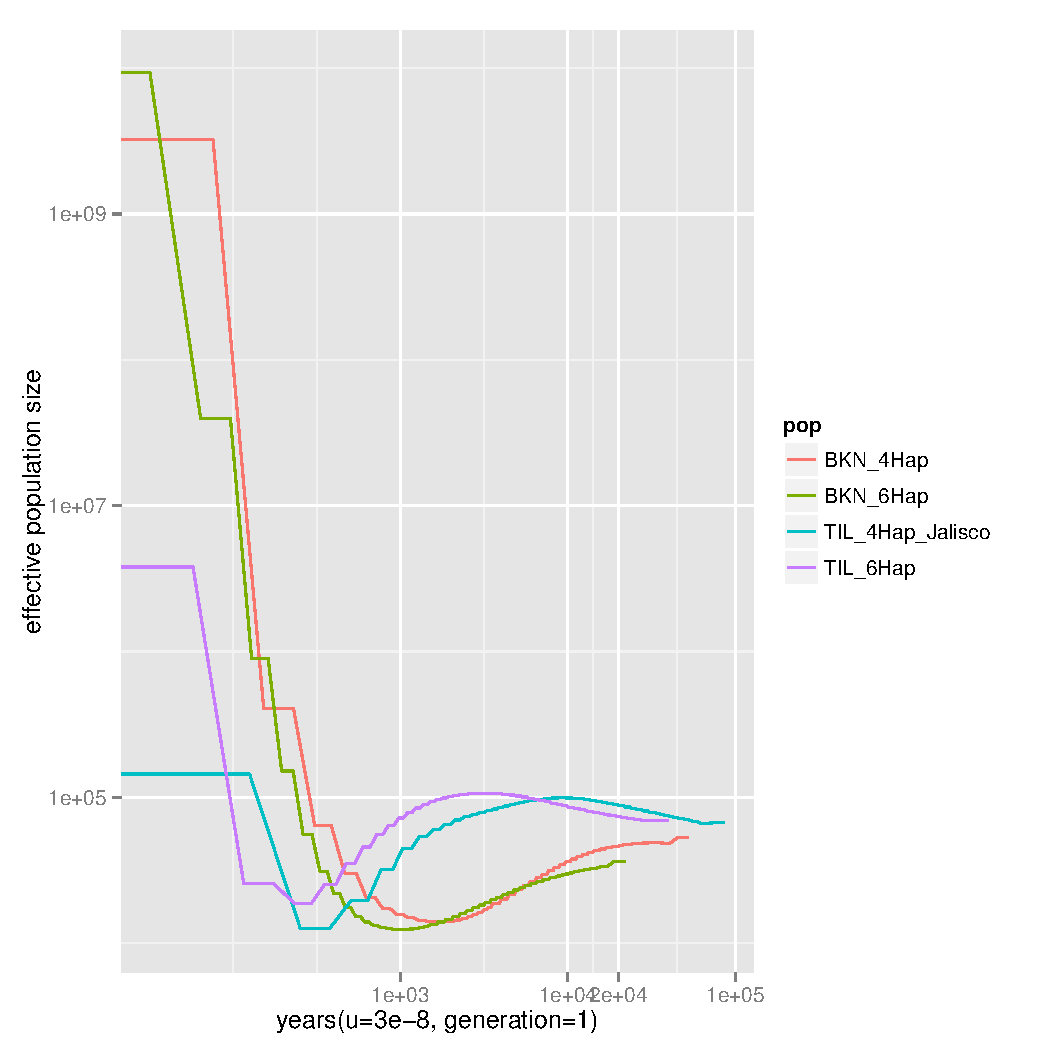
\includegraphics[width=.85\textwidth]{FigsAndFiles/BKN.TIL.msmc.pdf} \\
    \end{center}
\caption{\jri{need MSMC caption} \label{sFig:msmc}}
\end{figure}
\clearpage


\begin{figure}
  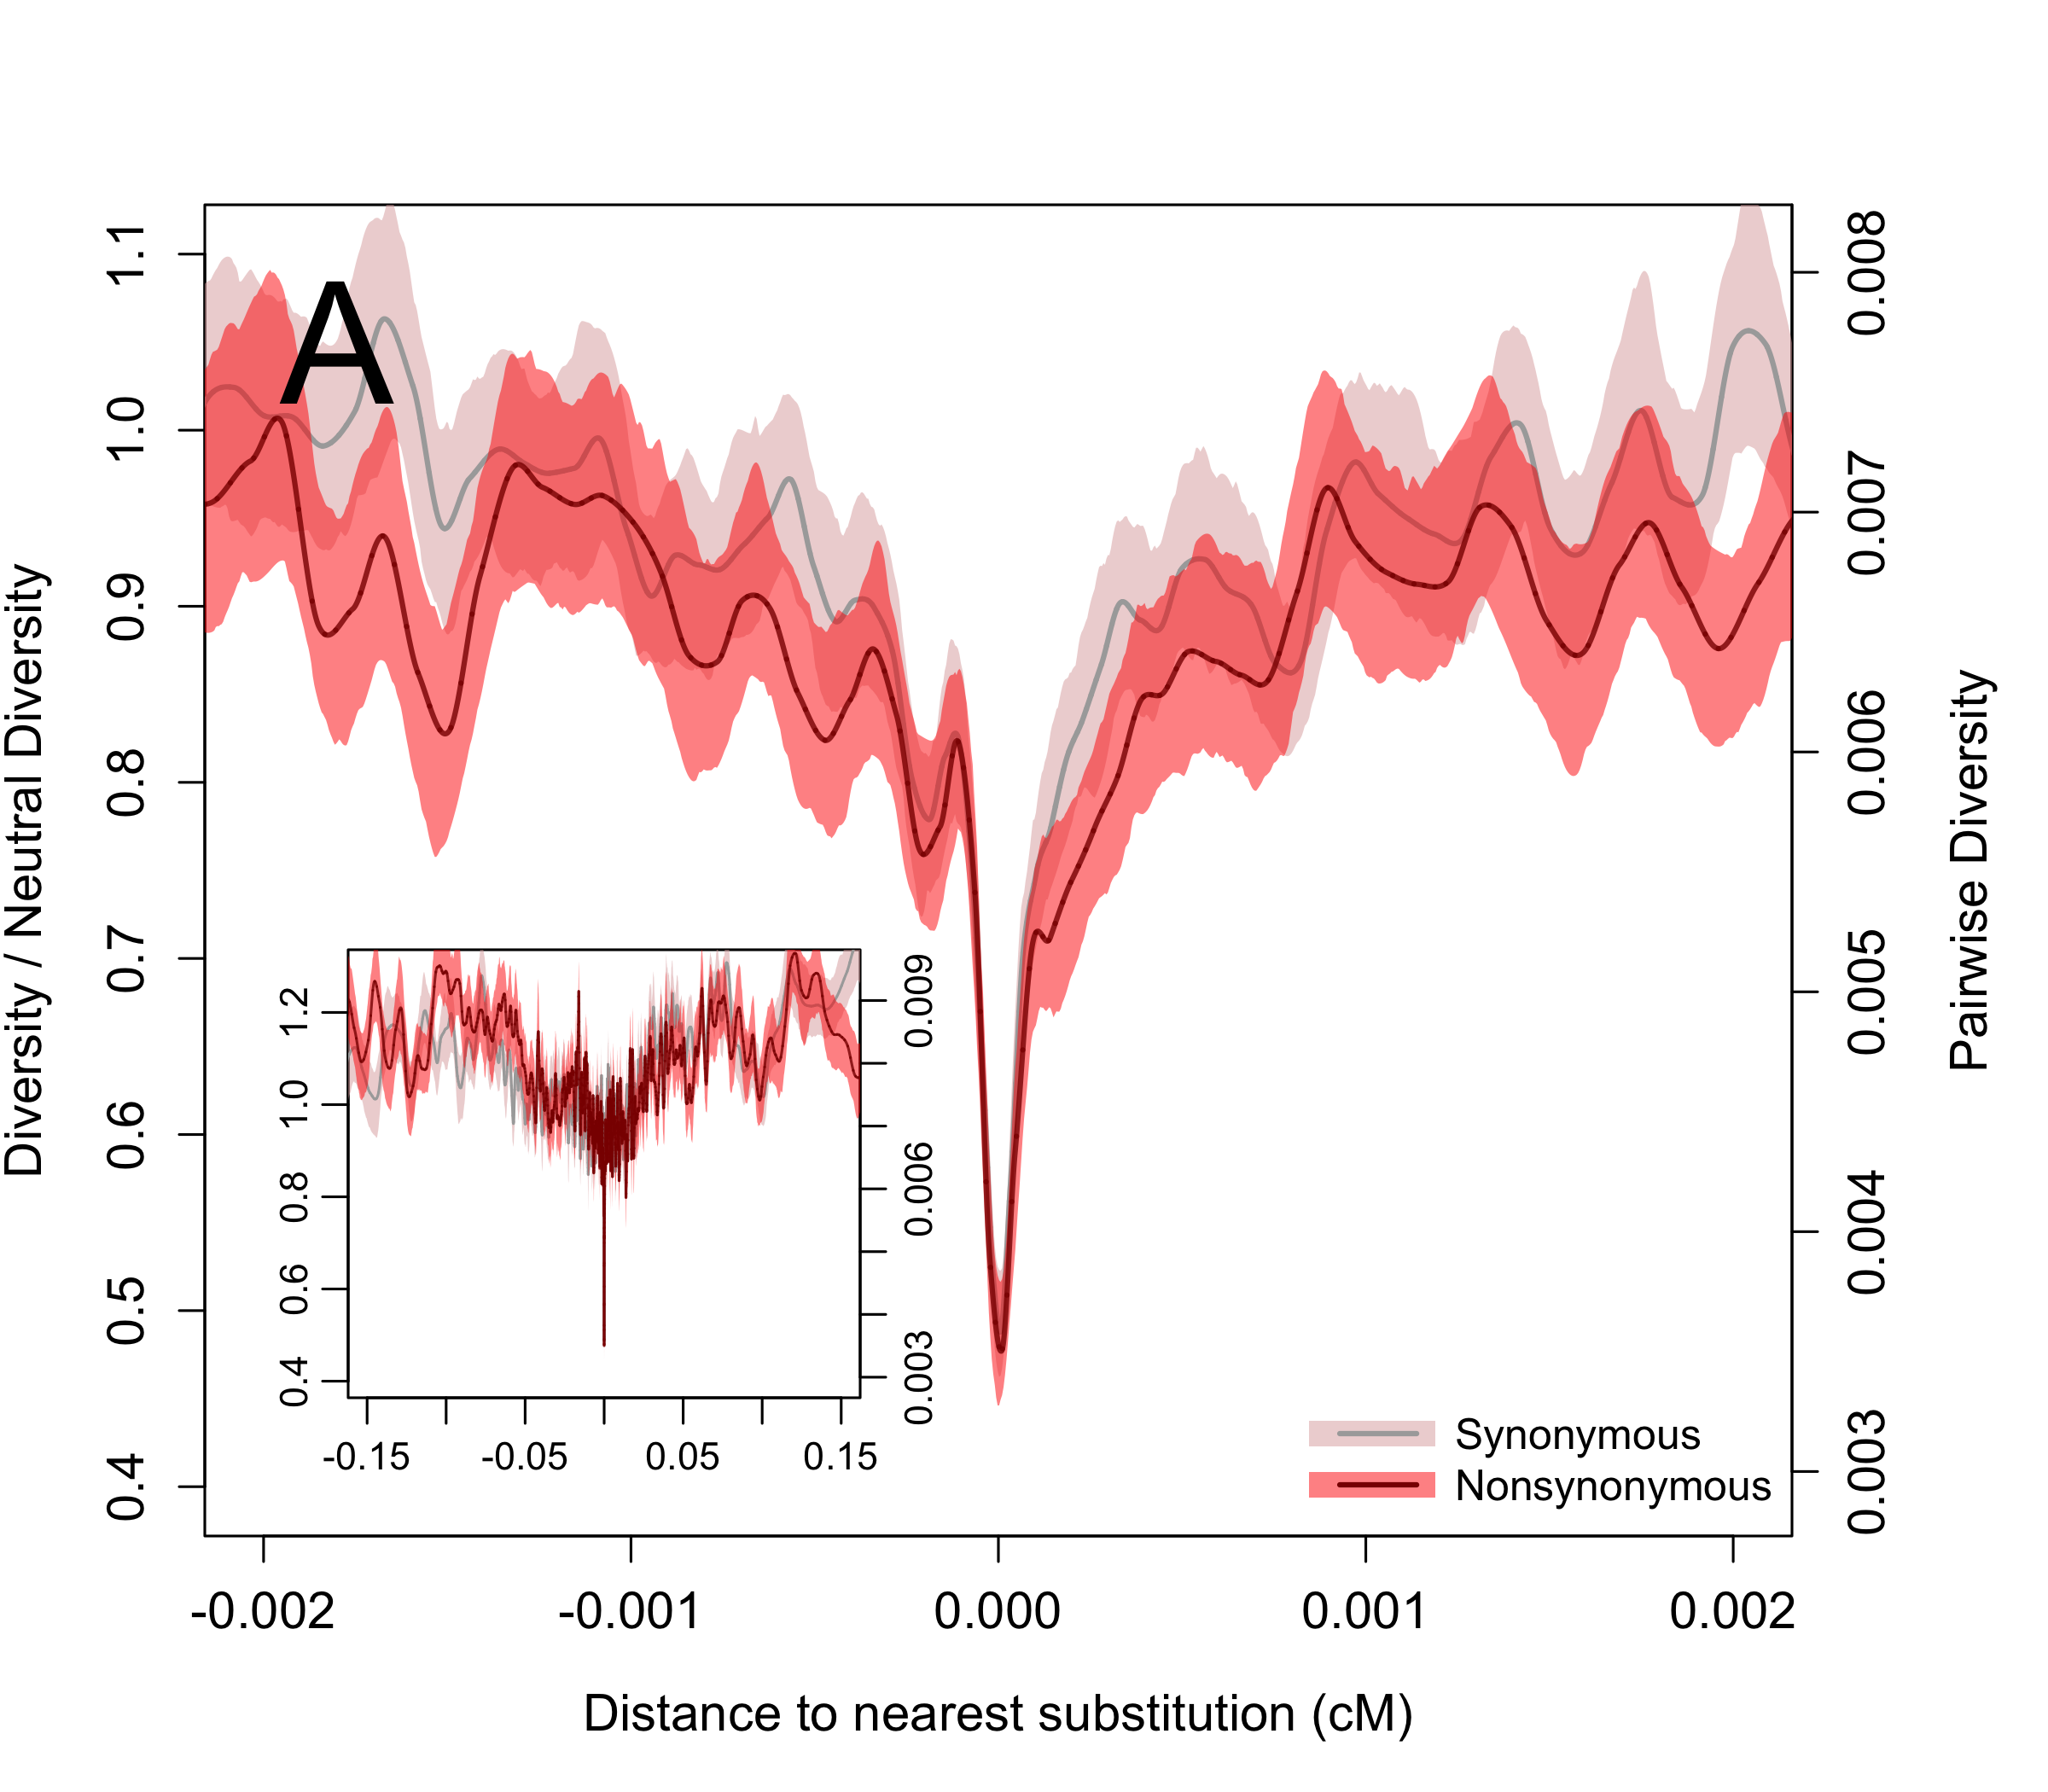
\includegraphics[width=.5\textwidth]{FigsAndFiles/plotDiversity_TvM_Conserved_Significance_June.png}
  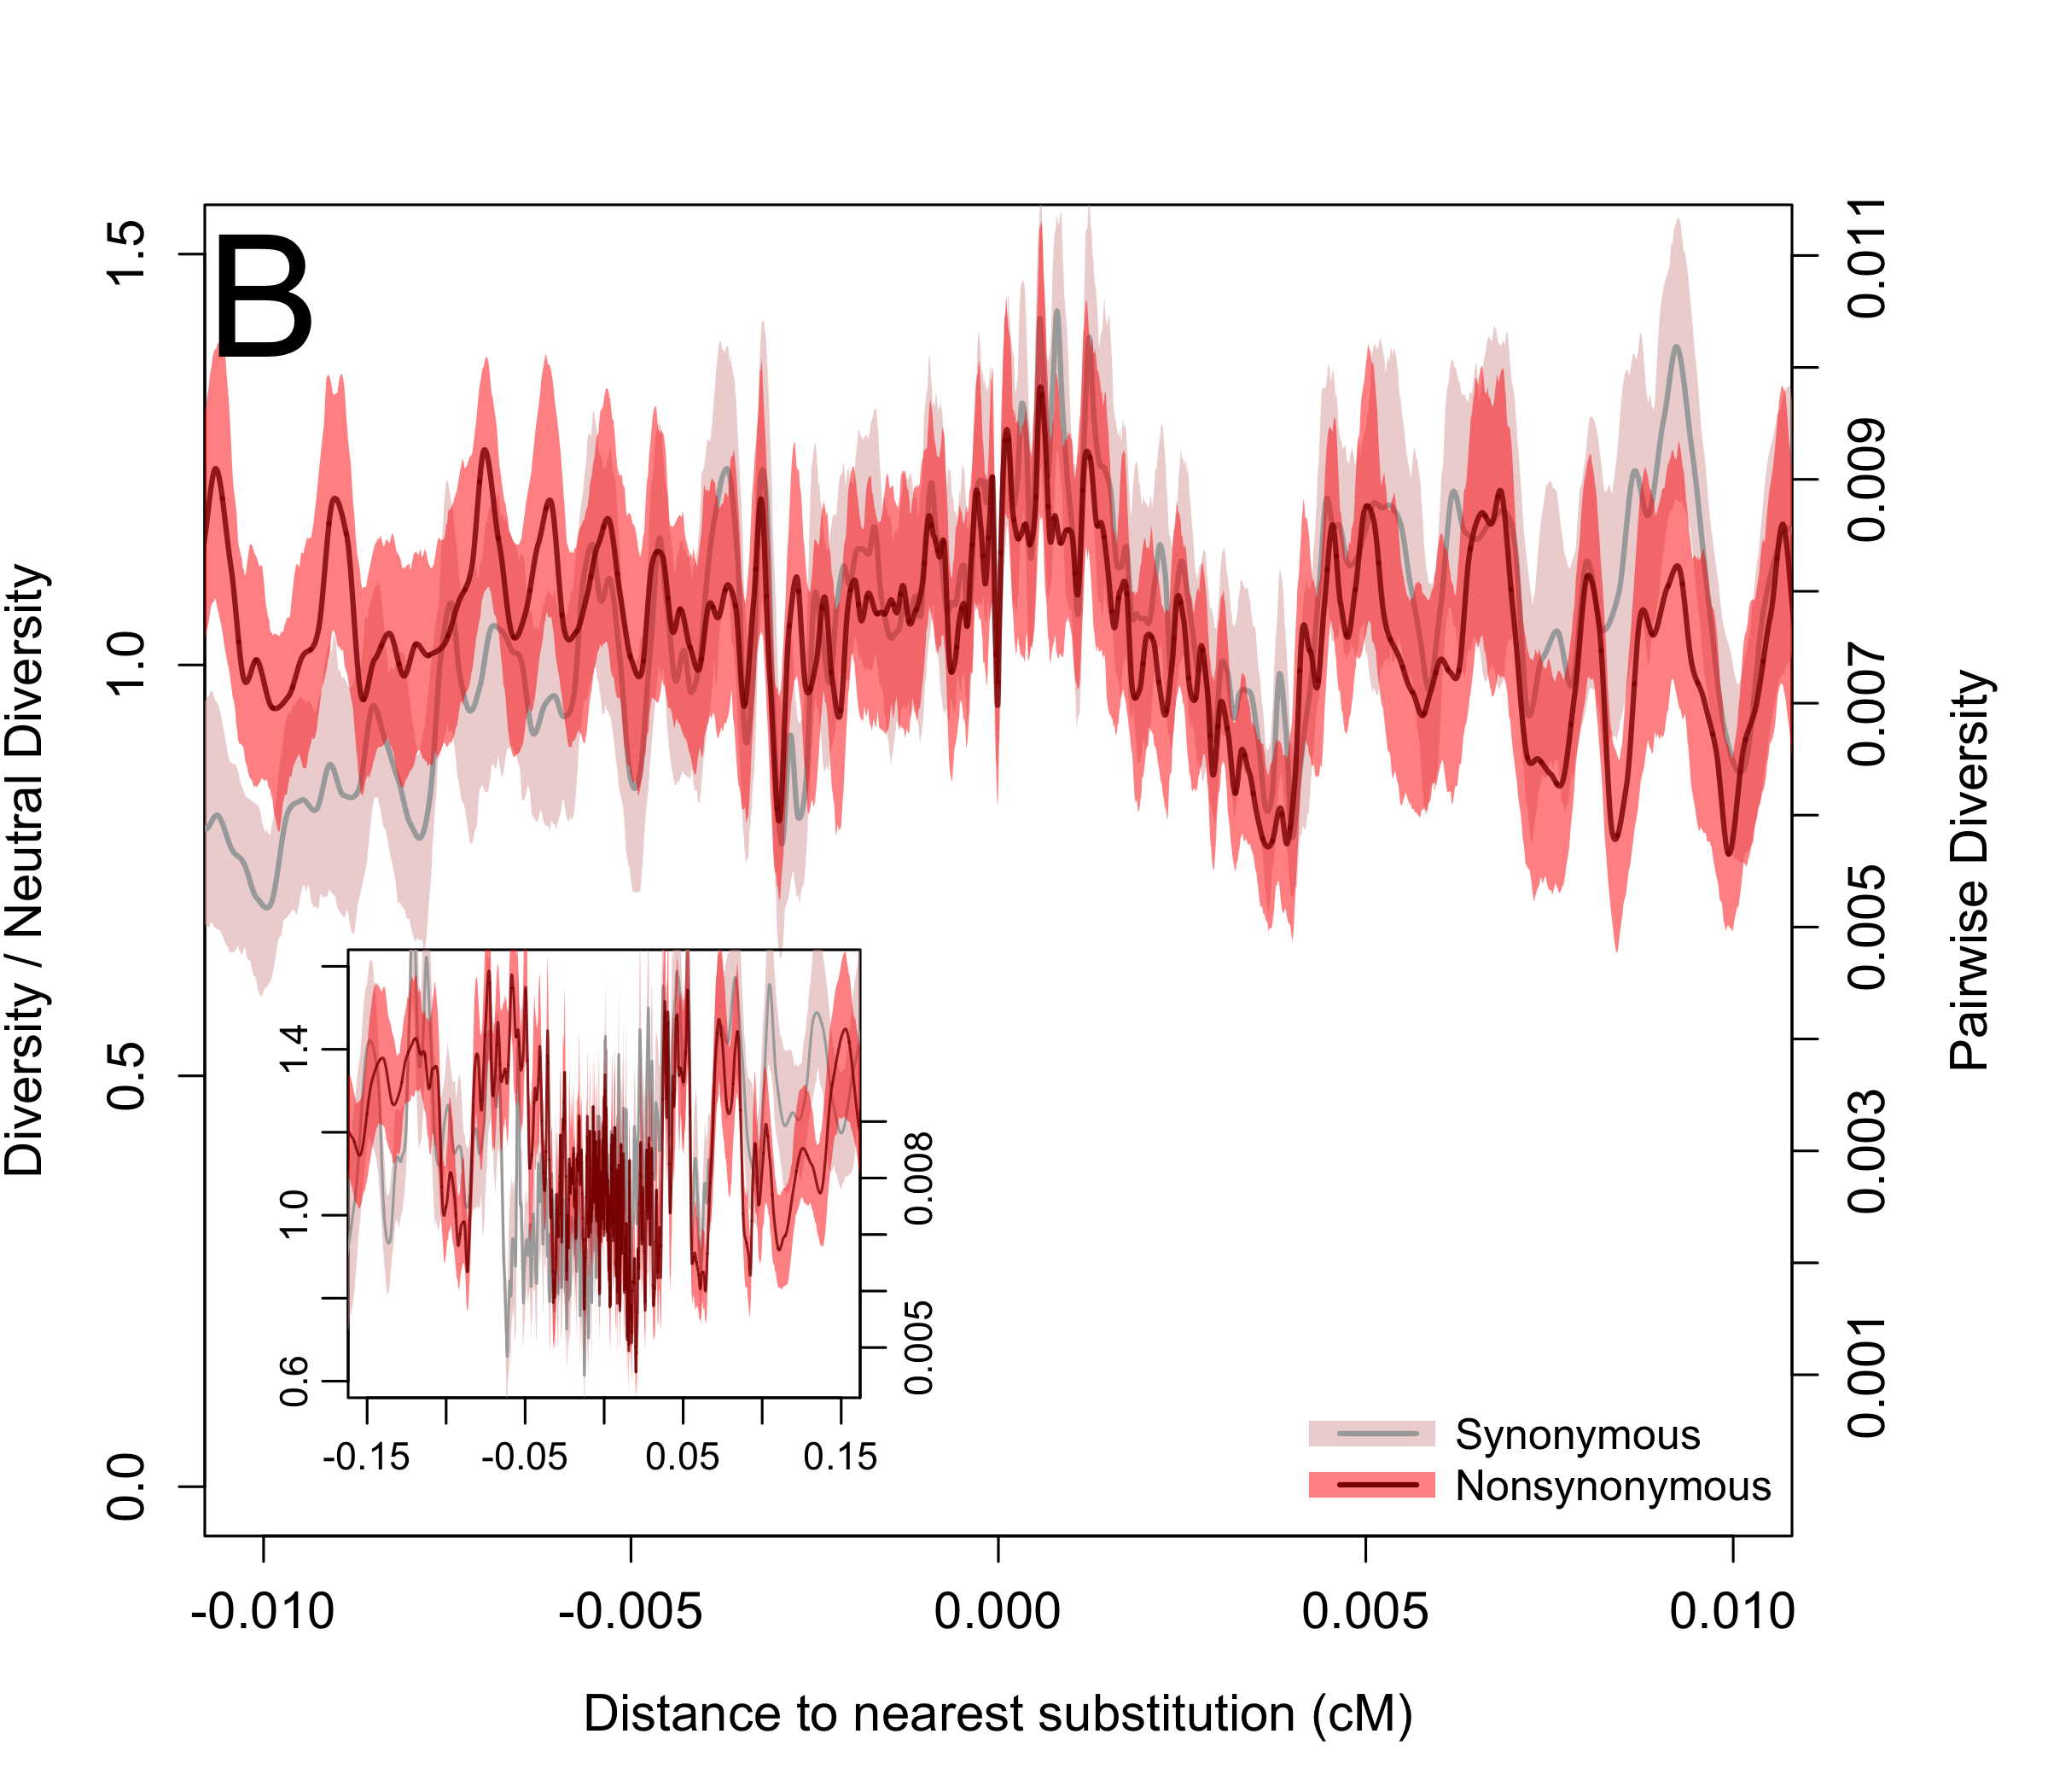
\includegraphics[width=.5\textwidth]{FigsAndFiles/plotDiversity_TvM_Unconserved_Significance_June.png}
\caption{ Pairwise diversity surrounding synonymous and nonsynonymous
  substitutions in maize at highly conserved (A) or unconserved (B) sites.  Bootstrap-based 95\% confidence intervals are depicted via shading. Inset plots depict a larger range on the x-axis. \label{sFig:consUncons}}
\end{figure}
\clearpage

\begin{figure}
  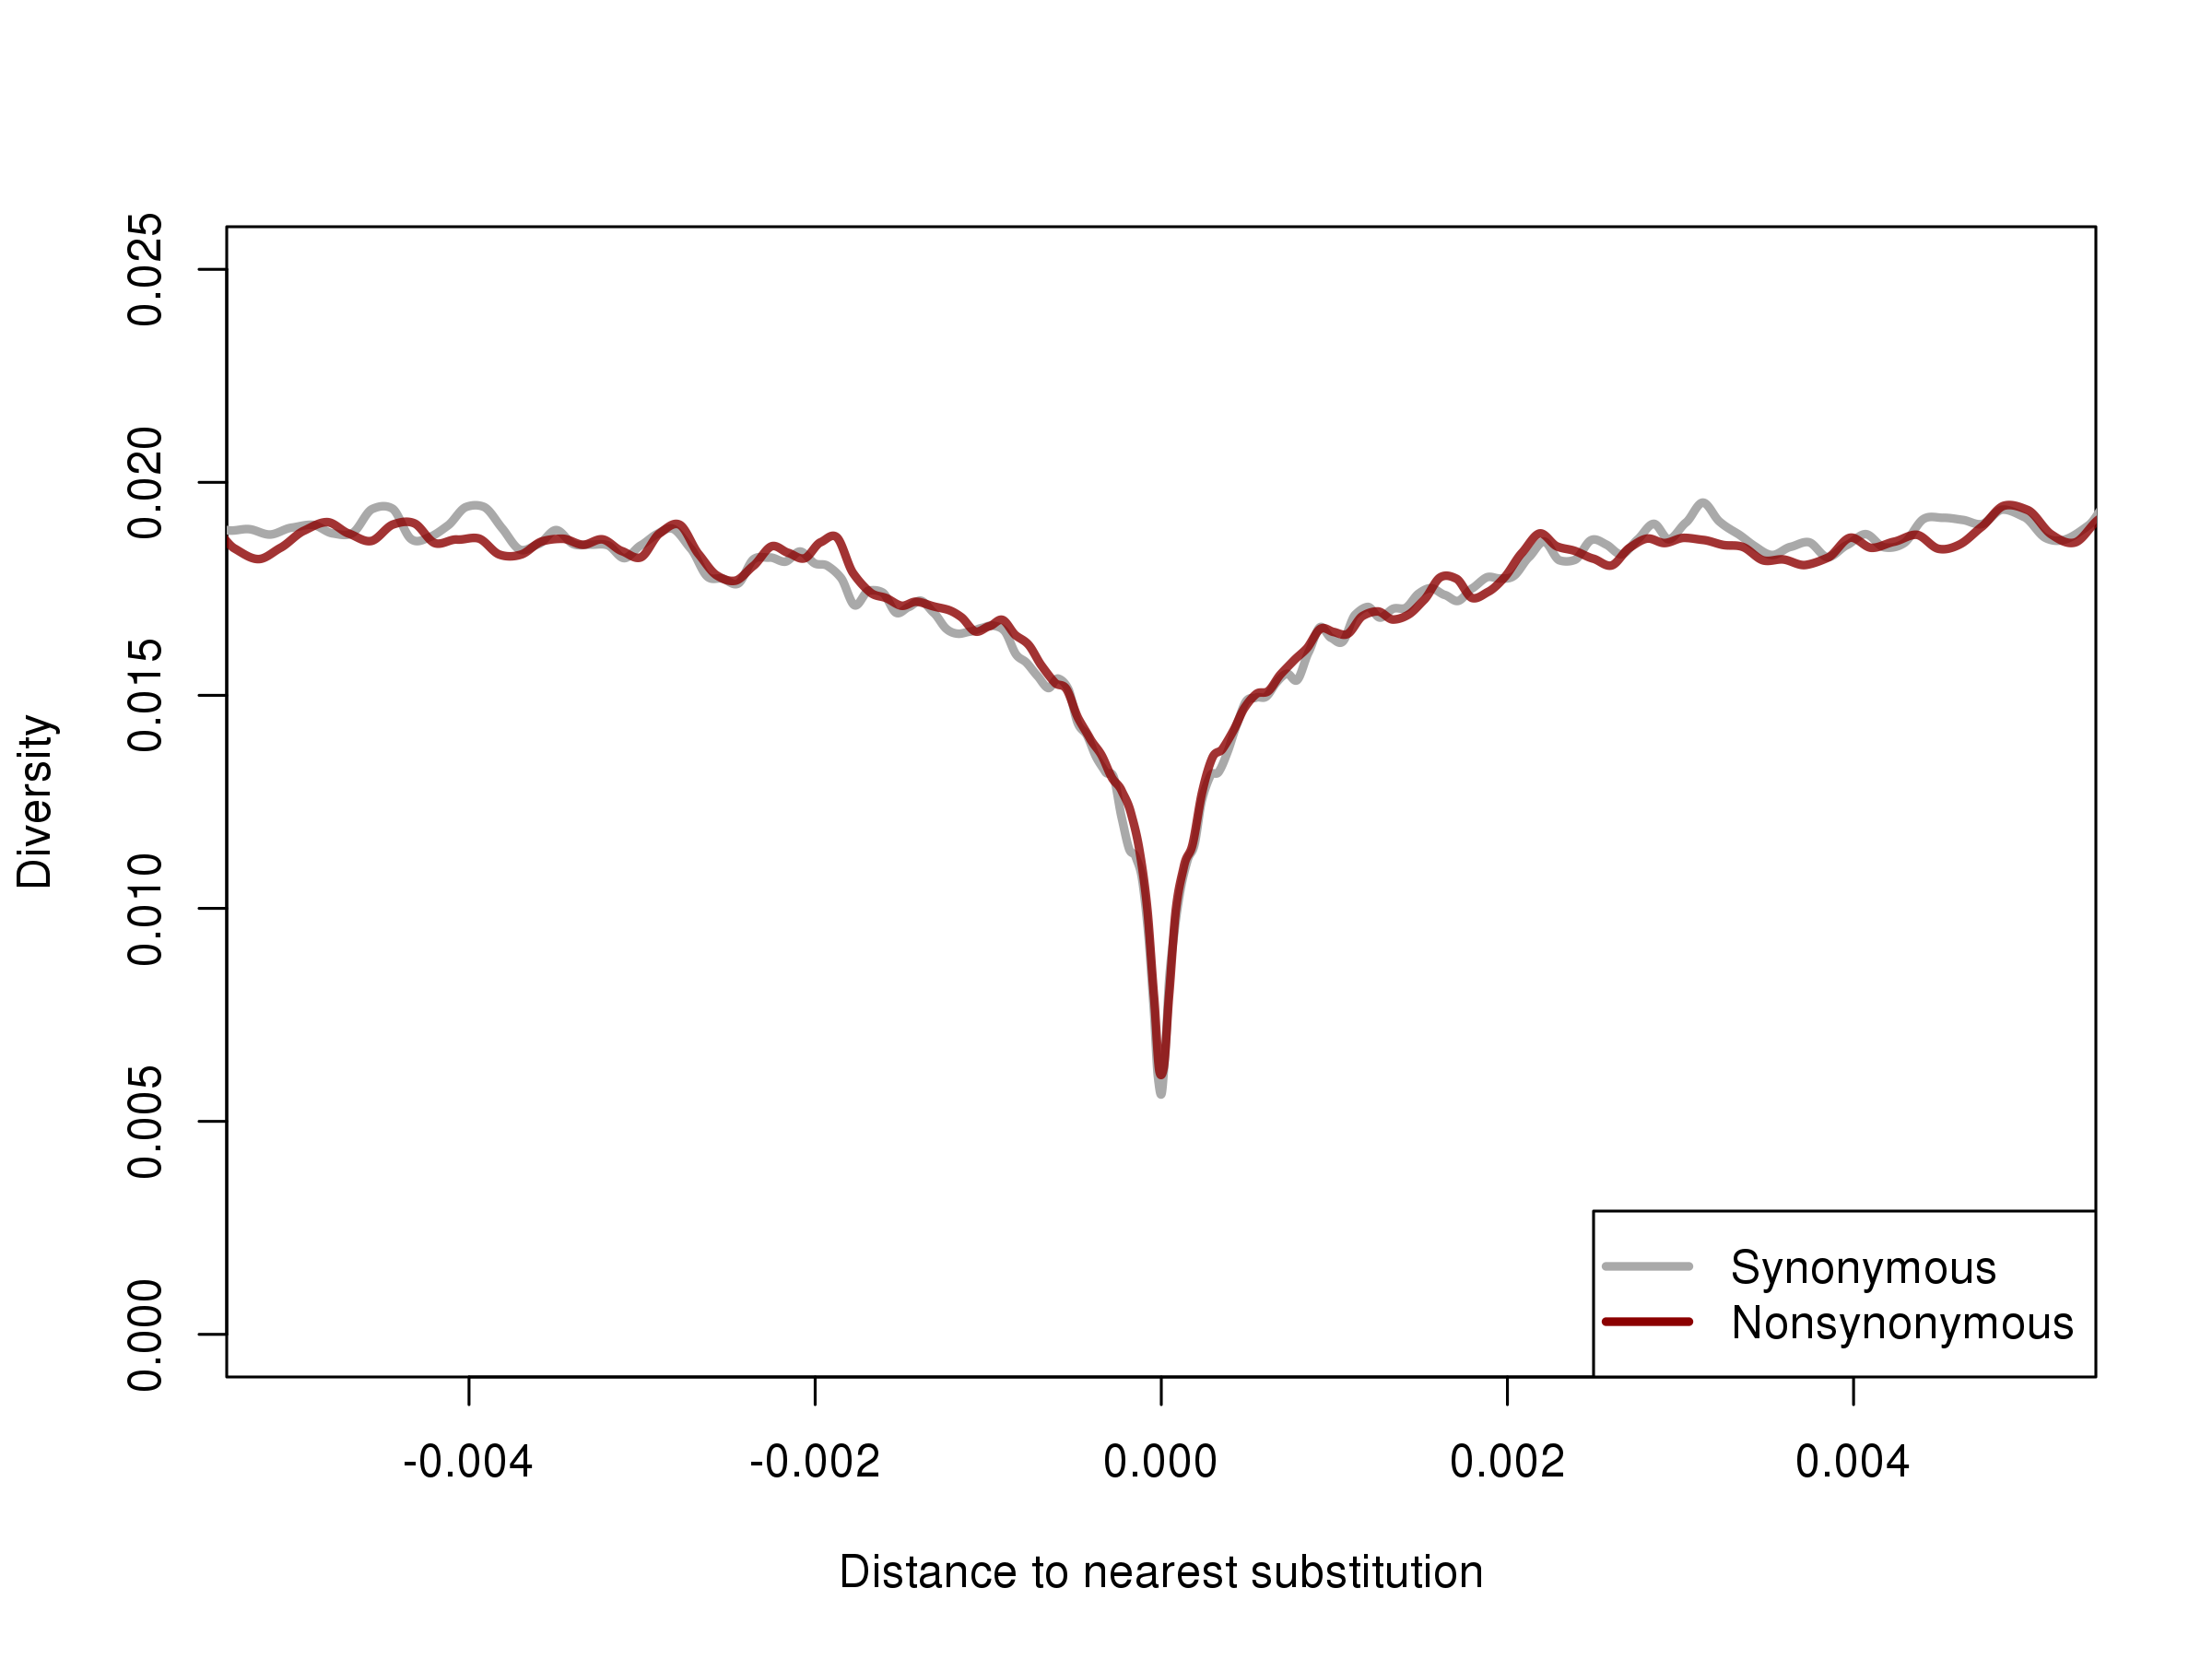
\includegraphics[width=\textwidth]{FigsAndFiles/plotDiversity_TvM_Singletons.png}
\caption{ Singleton diversity surrounding synonymous and nonsynonymous
  substitutions in maize. \label{sFig:singleton}}
\end{figure}
\clearpage


\begin{figure}
  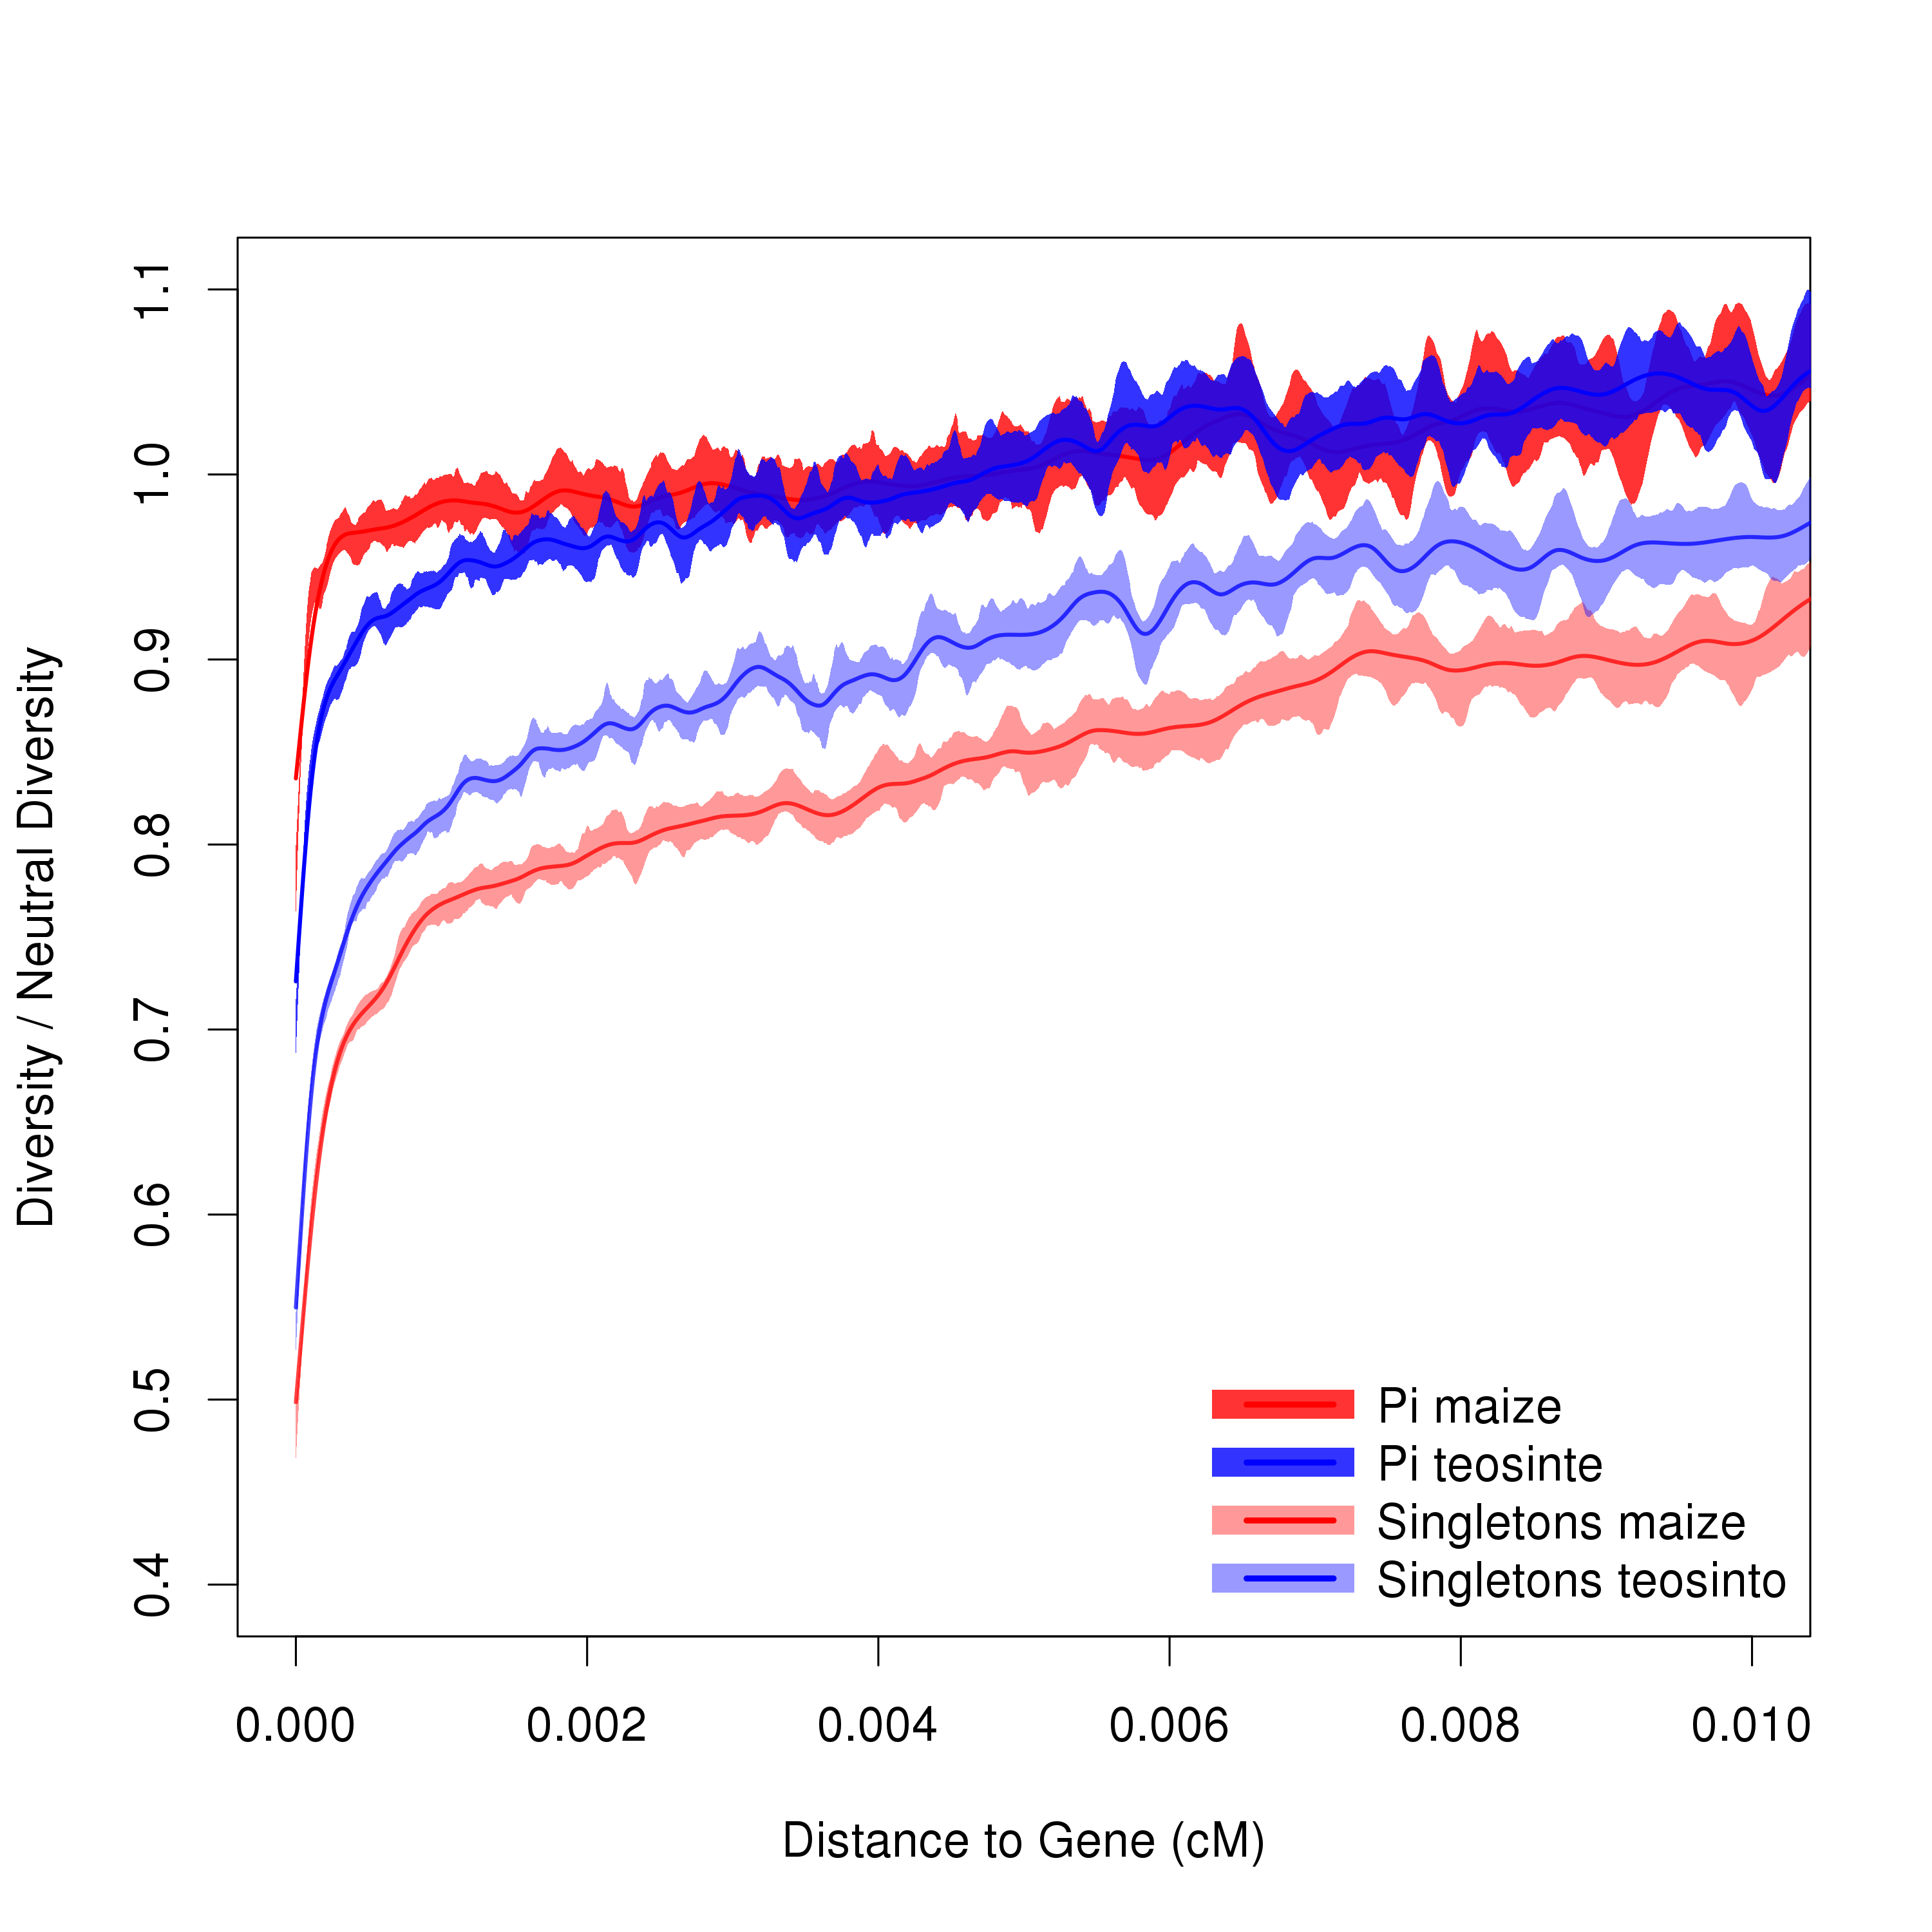
\includegraphics[width=\textwidth]{FigsAndFiles/distanceToGene_WithSignificance_Folded2_maizeAndTeoSingleVsPi.png}
\caption{ Relative diversity versus distance to nearest gene in maize and teosinte. Relative diversity is calculated by comparing to the mean diversity in all windows $\geq 0.02 cM$ from the nearest gene. Lines depict cubic smoothing splines with smoothing parameters chosen via generalized cross validation and shading depicts bootstrap-based 95\% confidence intervals.  \label{sFig:singletonPi}}
\end{figure}
\clearpage


\begin{figure}
  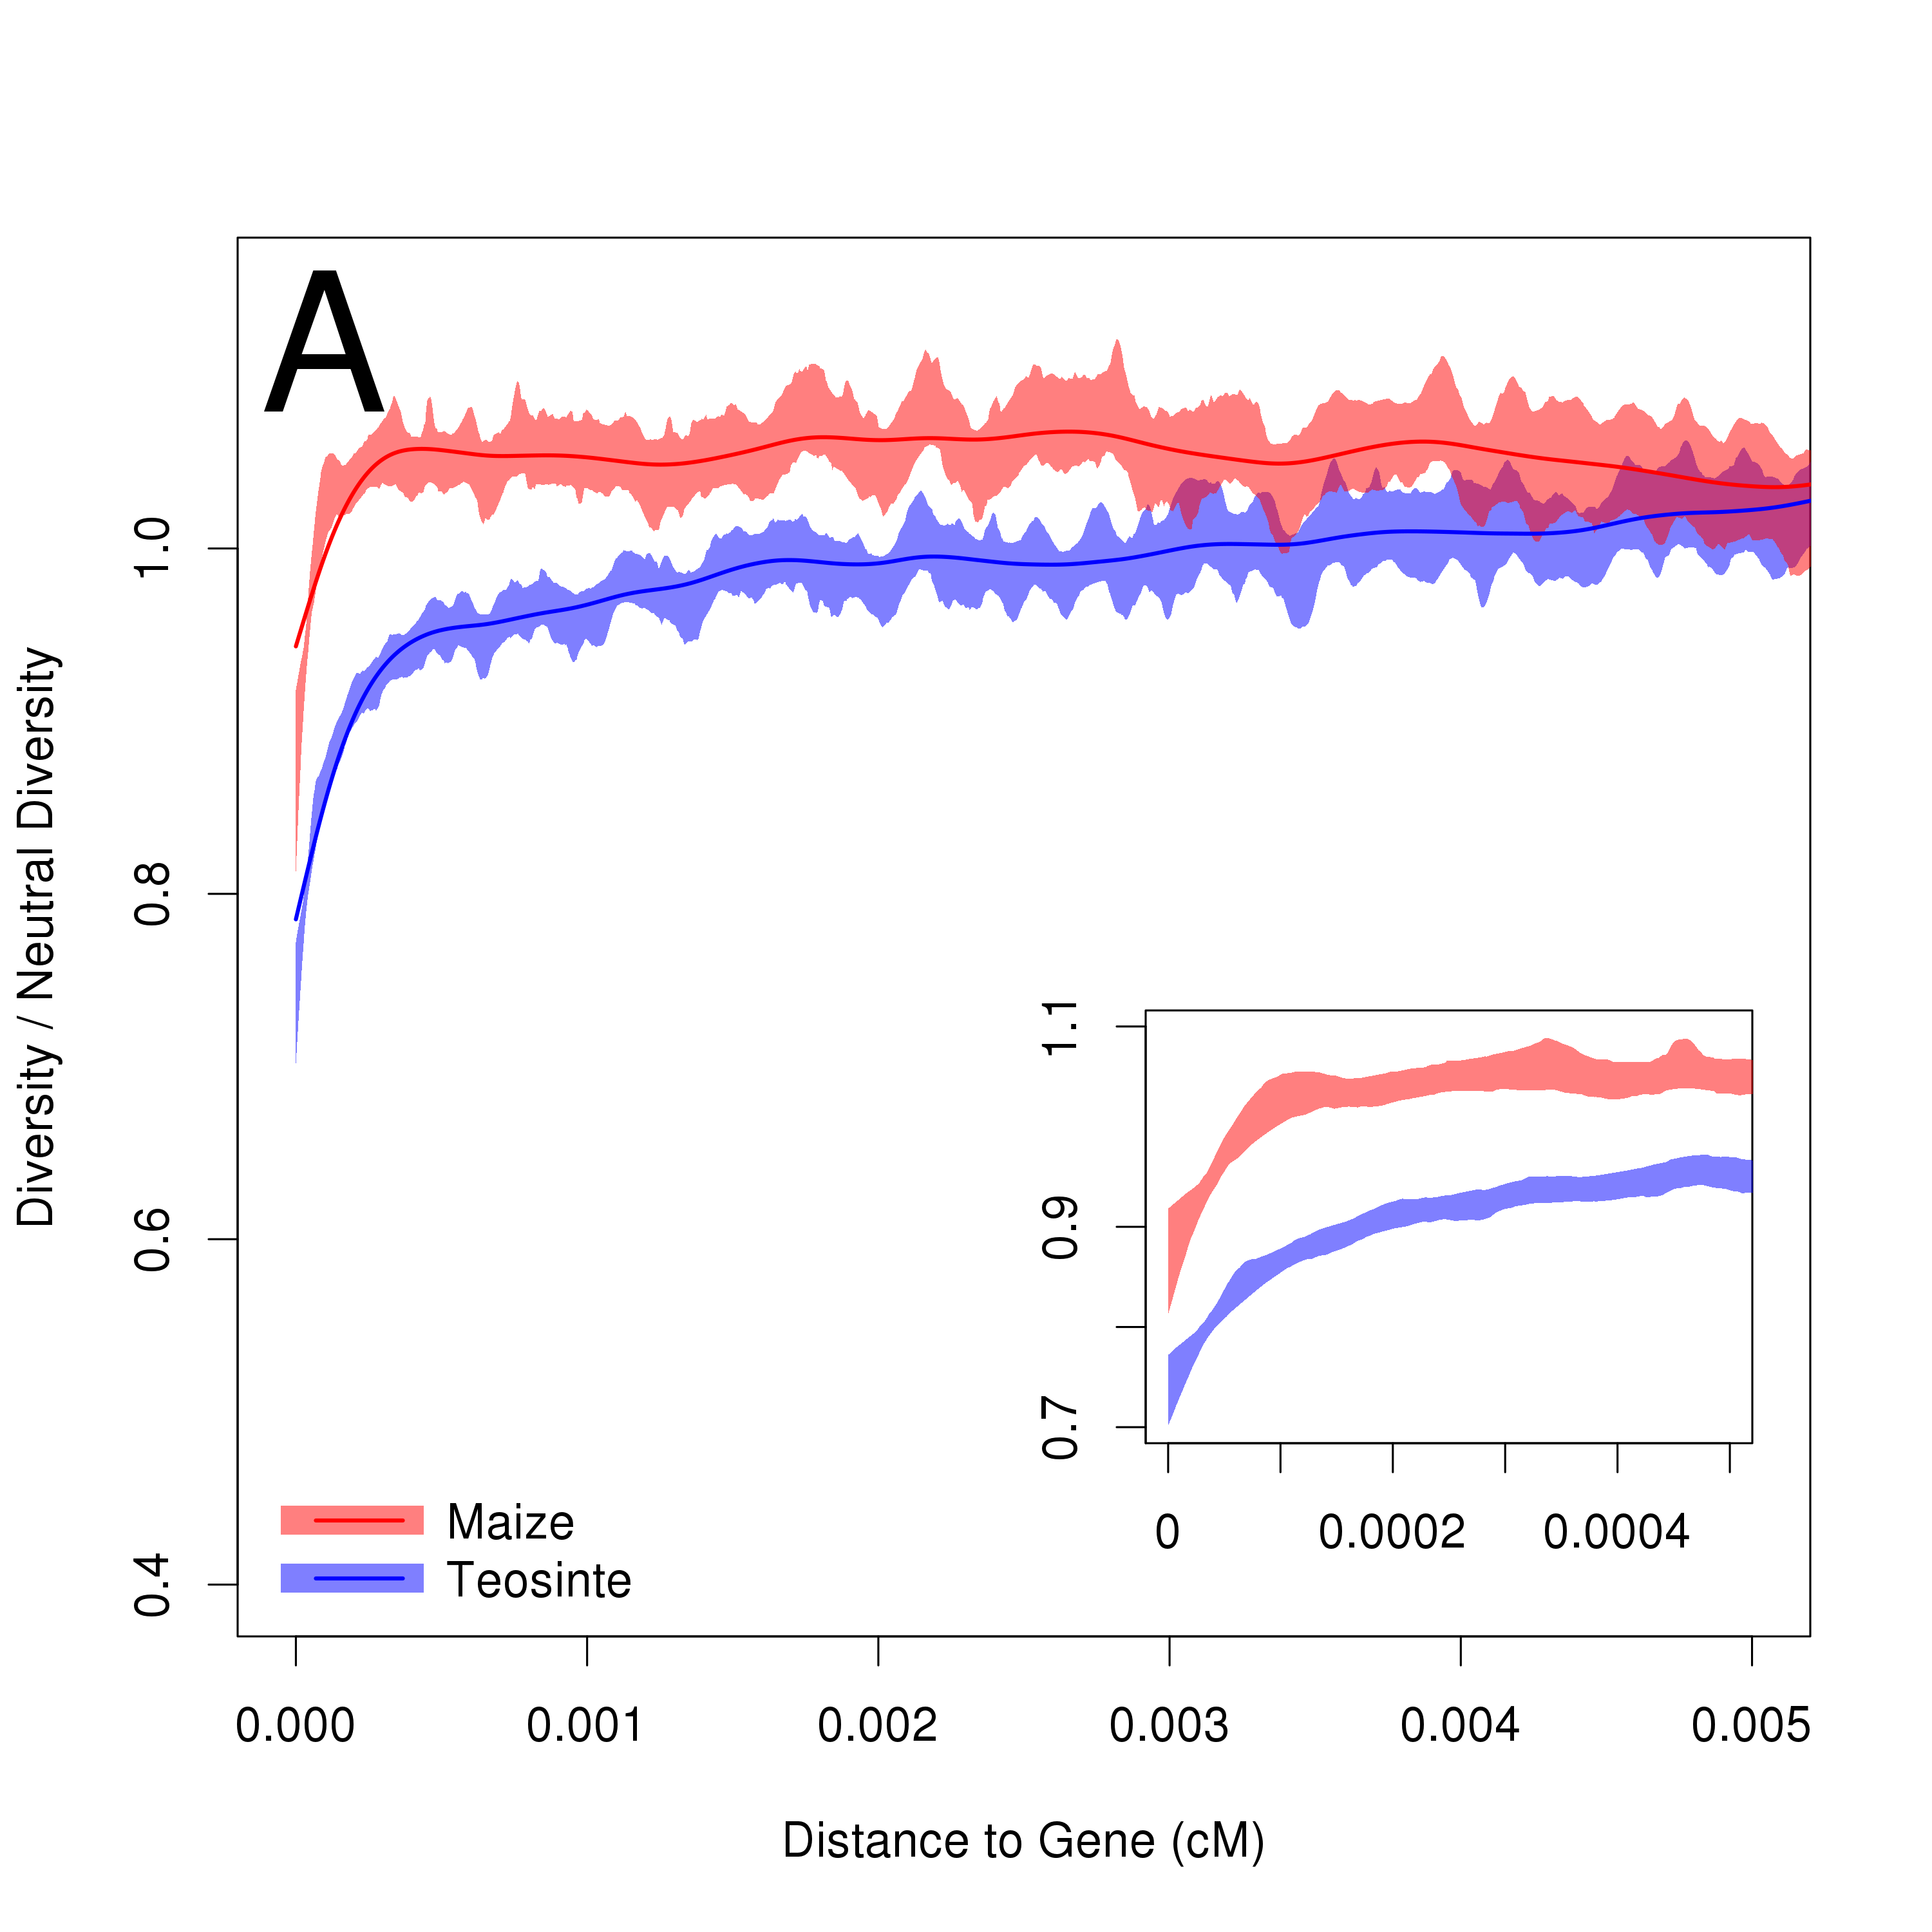
\includegraphics[width=.5\textwidth]{FigsAndFiles/distanceToGene_Unselected_manuscript.png}
    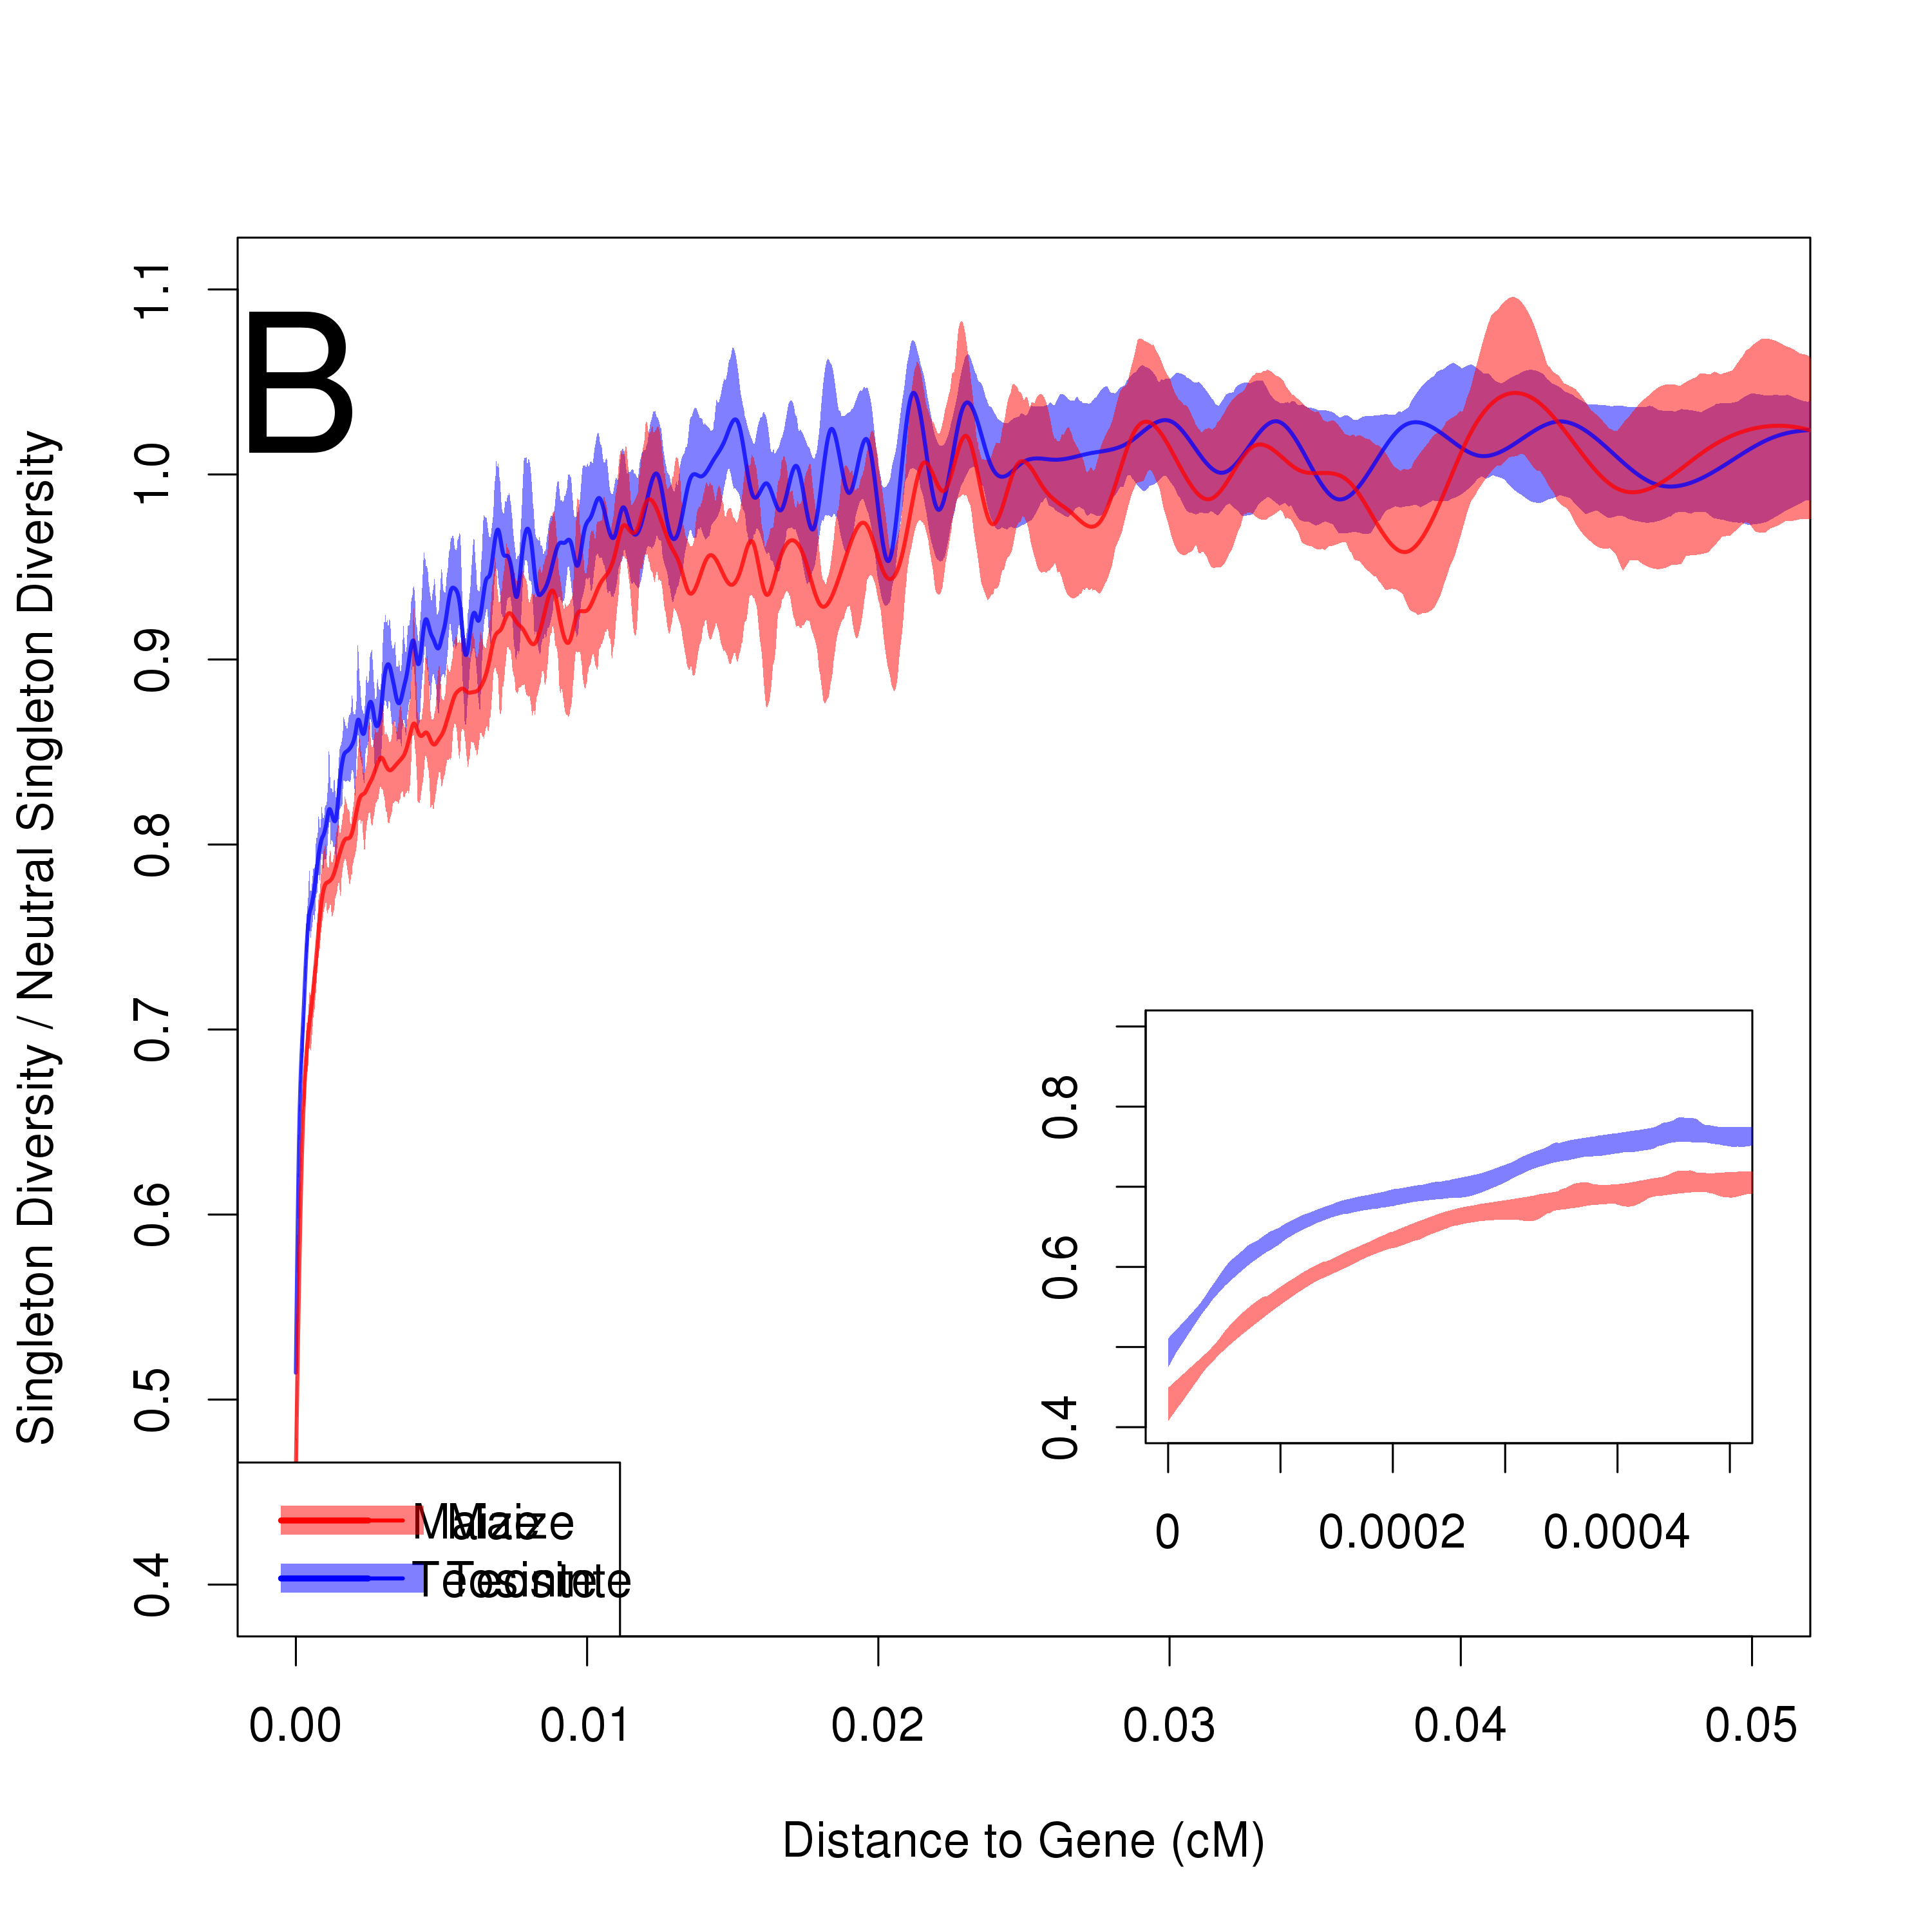
\includegraphics[width=.5\textwidth]{FigsAndFiles/distanceToGene_unselected_Singletons_manuscript.png}
\caption{ Relative level of diversity versus distance to the nearest gene, in maize and teosinte, based on only sites that do not show evidence of hard or soft sweeps according to H12. Two measures of diversity were investigated. {\bf A} displays pairwise diversity,
which is most influenced by intermediate frequency alleles and therefore depicts more ancient evolutionary patterns, and {\bf B} depicts singleton diversity, influenced by rare alleles and thus depicting evolutionary patterns in the recent past. Bootstrap-based 95\% confidence intervals are depicted via shading. Inset plots depict a smaller range on the x-axis. \label{sFig:H12}}
\end{figure}
\clearpage


\begin{figure}
  \begin{center}
  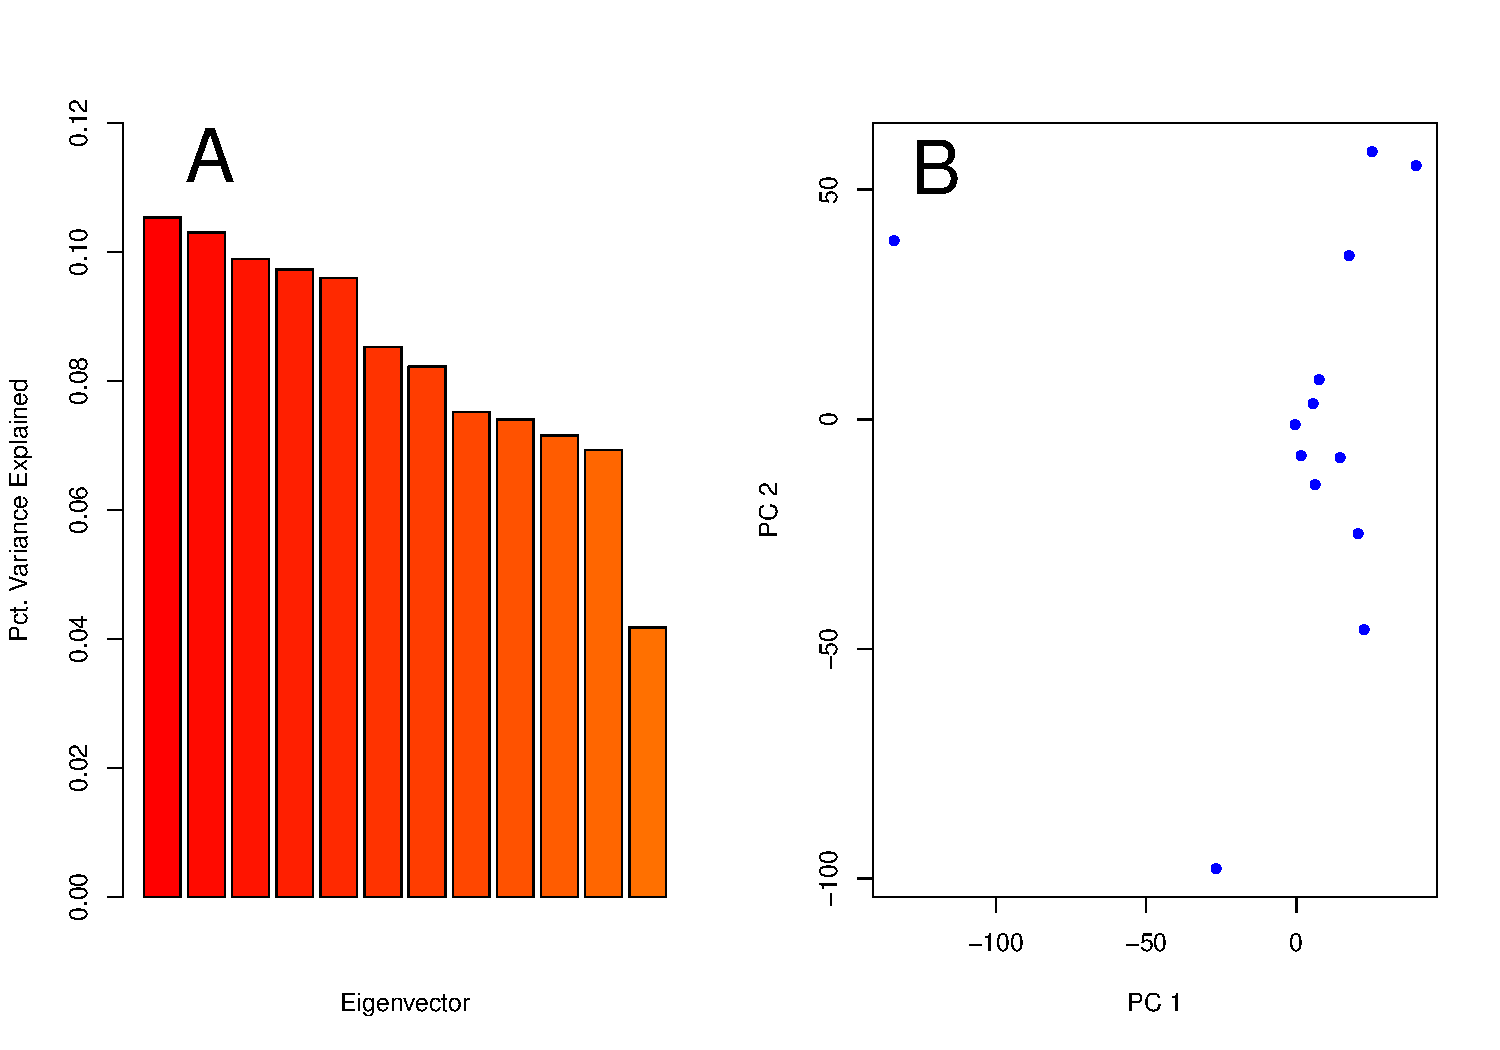
\includegraphics[width=.75\textwidth]{FigsAndFiles/tilPCA_aug.pdf}\\
  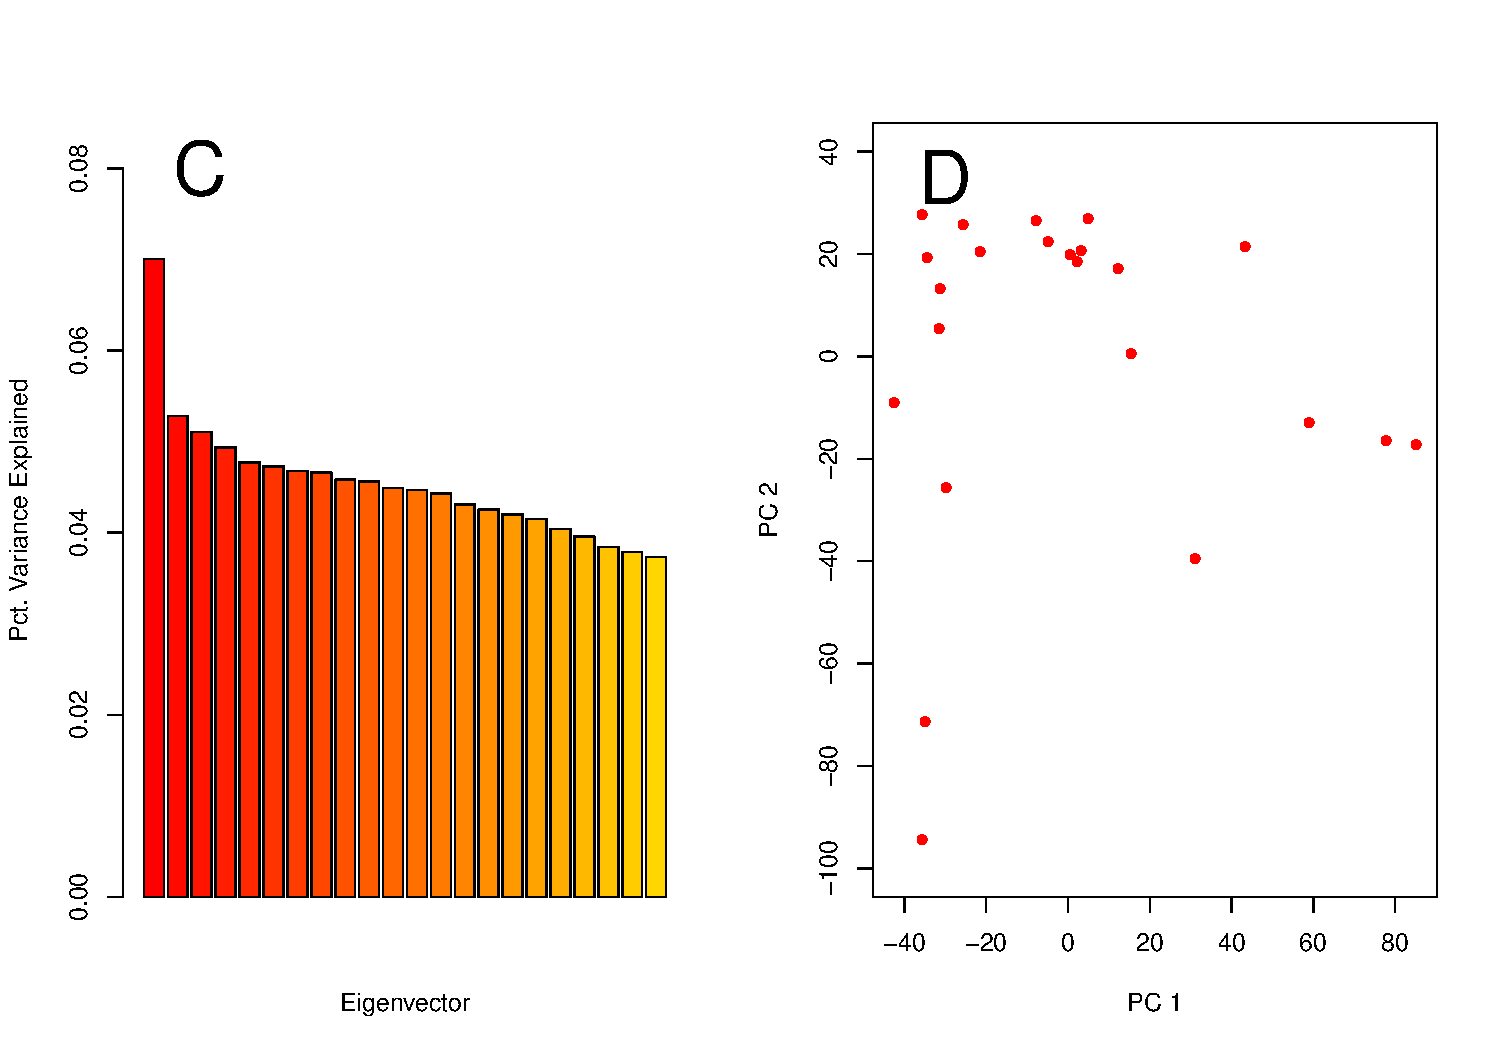
\includegraphics[width=.75\textwidth]{FigsAndFiles/bknPCA_aug.pdf}\\
  \end{center}
  \caption{Principal component analysis of teosinte and maize individuals to ensure that no close relatives were inadvertantly included in our study. Plots are based on a random sample of 10,000 SNPs. {\bf A:} Percentage of total variance explained by each principal component for teosinte. {\bf B:} PC1 vs PC2 for all 13 teosinte individuals. {\bf C:} Percentage of total variance explained by each principal component for maize. {\bf D:} PC1 vs PC2 for all 23 maize individuals. \label{sFig:PCA}}
\end{figure}
\clearpage


\begin{figure}
%  \begin{center}
  \begin{tabular}{c|c}
    \bf Maize & \bf Teosinte \\ \hline \hline
    BKN009 &  TIL01 \\
    BKN010 & TIL02 \\
    BKN011 & TIL03 \\
    BKN014 & TIL04-TIP454 \\
    BKN015 & TIL07 \\
    BKN016 & TIL09 \\
    BKN017 & TIL10 \\
    BKN018 & TIL11 \\
    BKN019 & TIL12 \\
    BKN020 & TIL14-TIP498 \\
    BKN022 & TIL15 \\
    BKN023 & TIL16 \\
    BKN025 & TIL17 \\
    BKN026 & \\
    BKN027 & \\
    BKN029 & \\
    BKN030 & \\
    BKN031 & \\
    BKN032 & \\
    BKN033 & \\
    BKN034 & \\
    BKN035 & \\
    BKN040 & \\
  \end{tabular} 
%  \end{center}
  \caption{ A list of maize and teosinte individuals included in this study. Sequencing and details were previously described by \jri{cite chia and lemmon}   \label{sTab:list} }
\end{figure}
\clearpage

\begin{figure}
  \def\arraystretch{2}
%  \begin{center}
  \begin{tabular}{l|c|c|c}
    \bf Parameter & \bf Initial value & \bf Upper bound & \bf Lower bound\\ \hline 
    $\frac{N_b}{N_a}$ & 0.02 & $1\times10^{-7}$ & 2 \\ 
    $\frac{N_{m}}{N_a}$ & 3 & $1\times10^{-7}$ & 200 \\
    $\frac{T_b}{2N_a}$ & 0.04 & 0  & 1 \\ 
    $\frac{M_{mt}}{N_a}$ & $1\times10^{-10}$ & $1\times10^{-7}$ & 0.001 \\
    $\frac{M_{tm}}{N_a}$ & $1\times10^{-10}$ & $1\times10^{-7}$ & 0.001 \\
  \end{tabular} 
%  \end{center}
  \caption{ Parameters, initial values, and boundaries used for model-fitting with $\delta\alpha\delta{i}$. Parameters are shown in the units utilized by $\delta\alpha\delta{i}$, although in the text simplified units are reported.   \label{sTab:dadi} }
    \def\arraystretch{1} % undo stretching
\end{figure}
\clearpage
 


\end{article}


\end{document}
